\chapter{Tema 2: Interacción en Física de Partículas}

\section{1. Partículas virtuales}

La descripción de la interacción entre partículas cargadas ha sufrido una evolución conceptual fundamental al pasar de la física clásica a la teoría cuántica de campos:

\begin{itemize}
    \item \textbf{Perspectiva clásica:} La interacción entre dos cargas $Q$ y $Q'$ se describe mediante el concepto continuo de \textit{campo electrostático} $\vec{E}$. La carga $Q$ genera un campo en todo el espacio y la carga $Q'$ experimenta una fuerza a distancia dada por $\vec{F} = Q' \vec{E}$.
    \item \textbf{Perspectiva cuántica:} La interacción ocurre mediante el intercambio discreto de cuantos del campo gauge (\textbf{bosones gauge}), que actúan como mediadores de la fuerza. Durante el proceso de dispersión entre $Q$ y $Q'$, se produce una transferencia de cuadrimomento $q^\mu = p^\mu - {p'}^\mu$ a través del intercambio de una \textbf{partícula virtual}.
\end{itemize}

\begin{figure}[htbp]
    \centering
    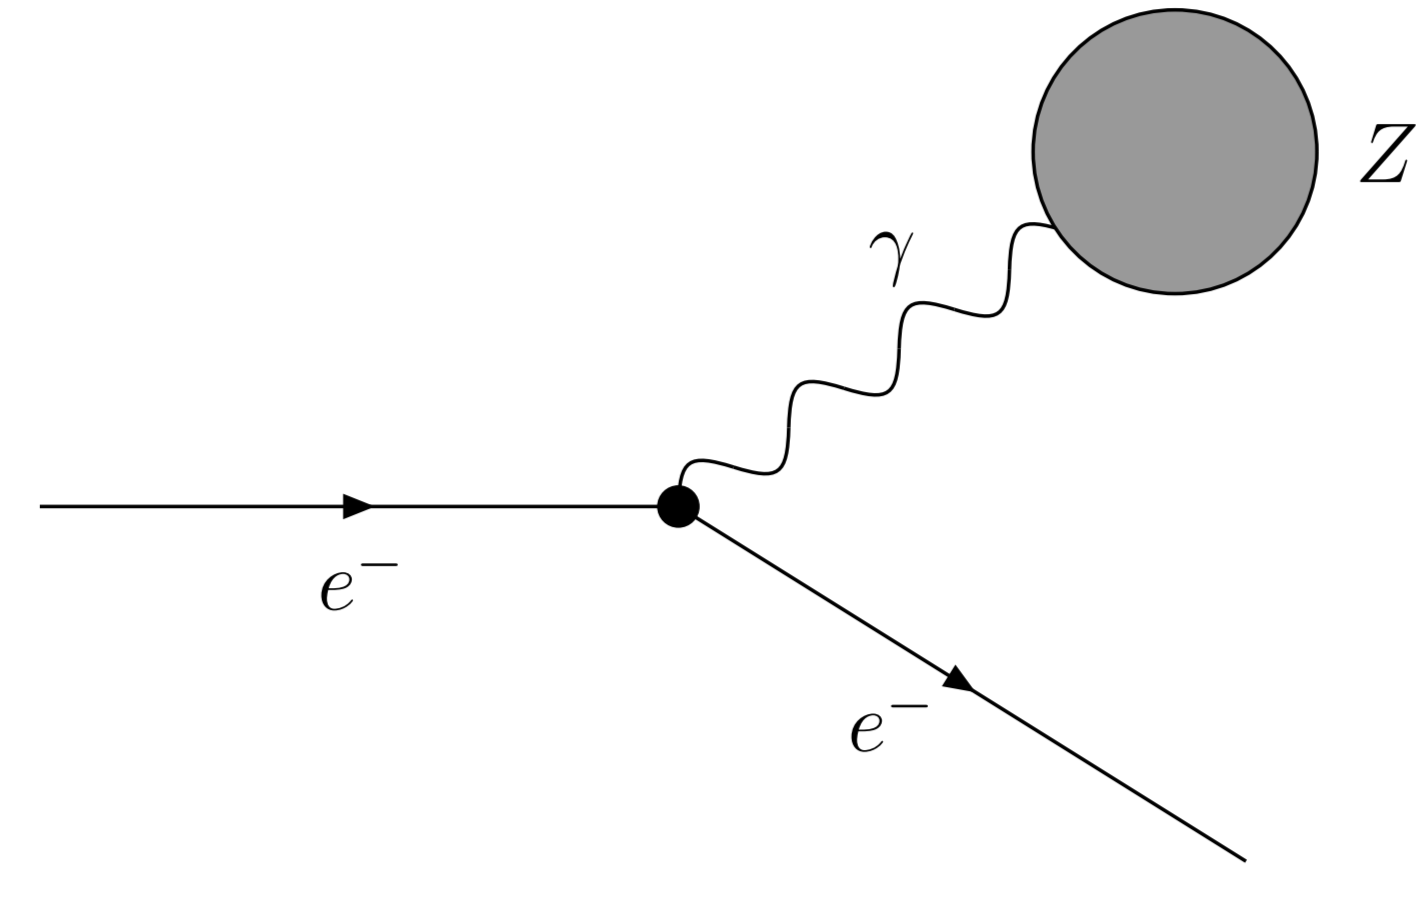
\includegraphics[width=0.85\textwidth]{imagenes/tema2/T2_1.png}
    \caption{Comparación entre la descripción clásica (campo y fuerza a distancia) y la descripción cuántica (intercambio de un bosón gauge virtual con transferencia de momento $\vec{q} = \vec{p} - \vec{p}'$) de la interacción electromagnética.}
    \label{fig:clasica_cuantica}
\end{figure}

\subsection*{Recordatorio: Acoplamiento electromagnético mínimo}

Para comprender la dinámica subyacente en el vértice de interacción, recordemos el comportamiento de una partícula no relativista de carga $q$ y masa $m$ bajo un potencial central $V(r)$. El hamiltoniano del sistema libre es:
\begin{equation}
    H_0 = \frac{p^2}{2m} + V(r)
\end{equation}

Al introducir la presencia de un campo electromagnético caracterizado por un potencial vector $\vec{A}(\vec{r}, t)$, se aplica la sustitución gauge o acoplamiento mínimo $\vec{p} \to \vec{p} - q\vec{A}$:
\begin{align}
    H &= \frac{(\vec{p} - q\vec{A})^2}{2m} + V(r) \nonumber \\
    &= \frac{p^2}{2m} + V(r) - \frac{q}{2m} (\vec{p} \cdot \vec{A} + \vec{A} \cdot \vec{p}) + \frac{q^2 A^2}{2m}
\end{align}

Tratando el campo en el gauge de Coulomb ($\nabla \cdot \vec{A} = 0$), el operador momento conmuta con el potencial vector, $[\vec{p}, \vec{A}] = -i\hbar \nabla \cdot \vec{A} = 0$, de modo que $\vec{p} \cdot \vec{A} = \vec{A} \cdot \vec{p}$. Por otro lado, en el régimen de campos débiles, el término cuadrático $\frac{q^2 A^2}{2m}$ es de orden superior en la constante de acoplamiento y resulta totalmente despreciable frente al término lineal. Así, el hamiltoniano de interacción electromagnética toma la forma:
\begin{equation}
    H_{\text{int}} = -\frac{q}{m} \vec{p} \cdot \vec{A}
\end{equation}
donde el potencial vector $\vec{A}(\vec{r}, t) \propto e^{i(\vec{k} \cdot \vec{r} - \omega t)}$ describe la emisión o absorción de cuantos de radiación de vector de onda $\vec{k}$.

\subsection*{Prohibición cinemática de la emisión libre de fotones reales}

Estudiemos la posibilidad cinemática de que un electrón libre emita un fotón real en un vértice de interacción simple. Supongamos un electrón inicialmente en reposo en el sistema del laboratorio que emite un fotón real $\gamma$ de cuadrimomento $k^\mu = (kc, \vec{k})$ y recula con momento $-\vec{k}$:
\begin{equation}
    e^-(mc^2, \vec{0}) \to e^-(E_k, -\vec{k}) + \gamma(kc, \vec{k})
\end{equation}

\begin{figure}[htbp]
    \centering
    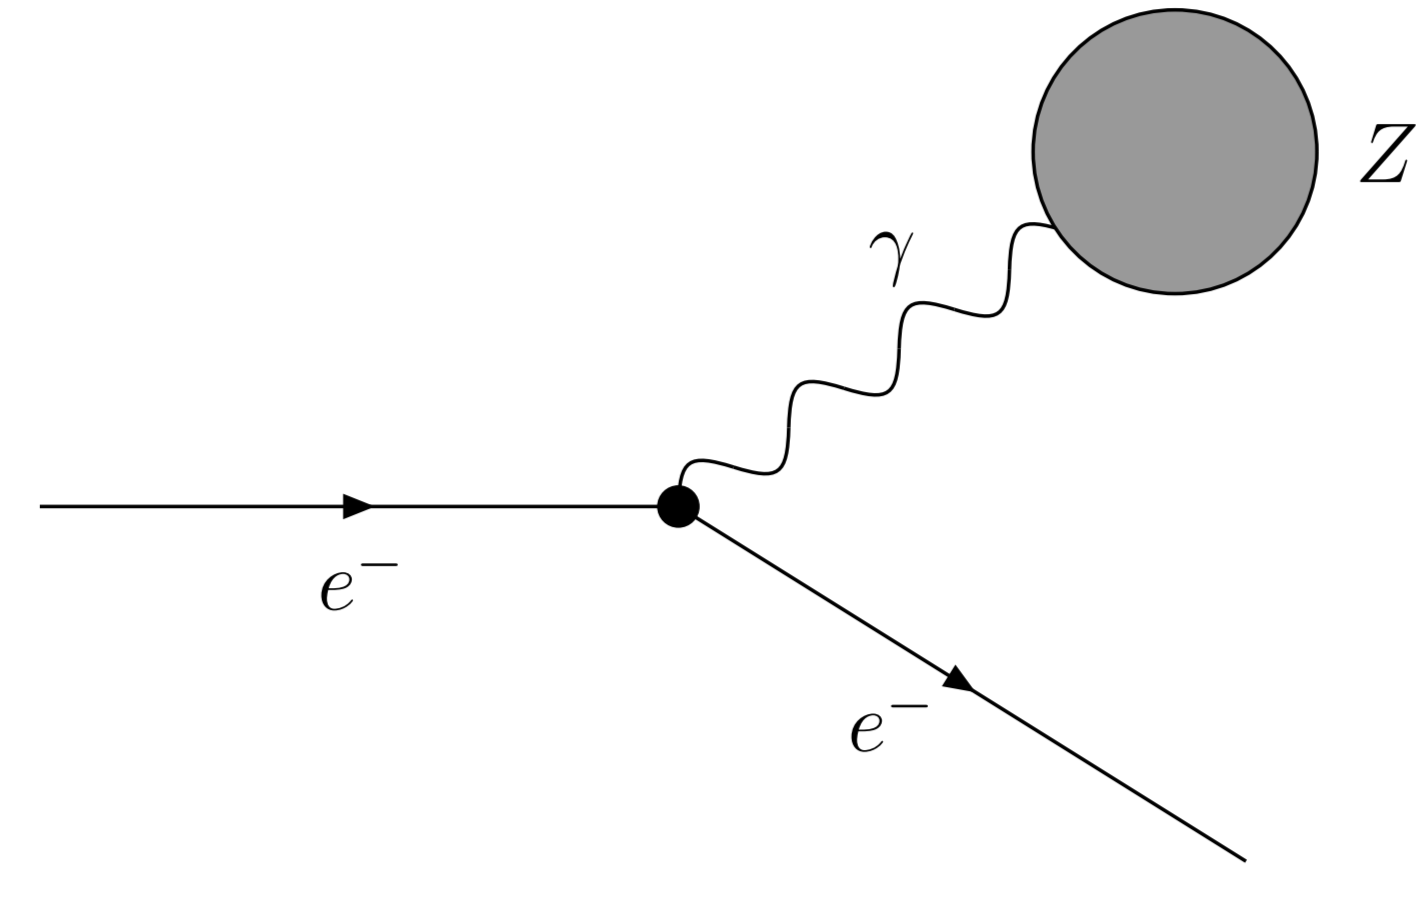
\includegraphics[width=0.45\textwidth]{imagenes/tema2/T2_1.png}
    \caption{Emisión de un fotón $\gamma$ por un electrón en presencia de un centro dispersor masivo de carga $Z$.}
    \label{fig:vertice_electron}
\end{figure}

Imponiendo la conservación del cuadrimomento total $P_i^\mu = P_f^\mu$:
\begin{enumerate}
    \item \textbf{Conservación del momento lineal:} $\vec{0} = \vec{p}_e + \vec{k} \implies \vec{p}_e = -\vec{k}$.
    \item \textbf{Conservación de la energía relativista:}
    \begin{equation}
        mc^2 = E_k + E_\gamma = \sqrt{m^2 c^4 + k^2 c^2} + kc
    \end{equation}
\end{enumerate}

Despejando el término radical y elevando al cuadrado ambos miembros:
\begin{align}
    mc^2 - kc &= \sqrt{m^2 c^4 + k^2 c^2} \nonumber \\
    (mc^2 - kc)^2 &= m^2 c^4 + k^2 c^2 \nonumber \\
    m^2 c^4 - 2 m c^3 k + k^2 c^2 &= m^2 c^4 + k^2 c^2 \nonumber \\
    -2 m c^3 k &= 0 \implies k \equiv |\vec{k}| = 0
\end{align}

\begin{concepto}[Prohibición cinemática del vértice libre]
La condición $k = 0$ implica que la energía del fotón debe ser estrictamente nula ($E_\gamma = 0$). En consecuencia, no existe fotón real emitido y el proceso $e^- \to e^- \gamma$ en el vacío está \textbf{estrictamente prohibido} por las leyes de conservación de energía y momento.
\end{concepto}

Para que un electrón emita un fotón real (como en el proceso de radiación de frenado o \textit{Bremsstrahlung}), es indispensable la presencia de un tercer cuerpo (por ejemplo, un centro nuclear de carga $Z$) que absorba parte del momento transferido y permita balancear la cinemática del proceso.

\subsection*{Naturaleza y propiedades de las partículas virtuales}

Para explicar la existencia de fuerzas mediadas sin violar la conservación cinemática en los vértices de interacción, la teoría cuántica introduce el concepto de \textbf{partícula virtual} (o bosón gauge virtual):

\begin{observacion}[Principio de incertidumbre y capa de masa]
\begin{itemize}
    \item \textbf{Violación transitoria de la energía:} De acuerdo con la relación de incertidumbre tiempo-energía de Heisenberg:
    \begin{equation}
        \Delta E \cdot \Delta t \ge \frac{\hbar}{2}
    \end{equation}
    la conservación de la energía puede "violarse" en una cantidad $\Delta E$ durante un intervalo de tiempo extremadamente corto $\Delta t \sim \frac{\hbar}{\Delta E}$. Durante este tiempo, la partícula virtual es creada y reabsorbida sin ser detectada directamente.
    
    \item \textbf{Capa de masa (\textit{Off-shell}):} Las partículas reales verifican de forma exacta la relación Einsteiniana de energía-momento $E^2 - p^2 c^2 = m^2 c^4$ (se dice que están \textit{on-shell} o sobre su capa de masa). Por el contrario, los bosones virtuales están \textbf{fuera de su capa de masa} (\textit{off-shell}):
    \begin{equation}
        q^2 = \frac{E^2}{c^2} - \vec{q}^2 \neq m^2 c^2
    \end{equation}
    
    \item \textbf{Inobservabilidad directa:} Una partícula virtual actúa únicamente como un estado intermedio en un diagrama de dispersión. Nunca puede registrarse directamente en un detector en el estado final asintótico. Si intentásemos medir directamente la partícula virtual durante el proceso, fijaríamos su trayectoria y energía, convirtiendo la fluctuación cuántica virtual en una violación observable de la conservación de la energía, lo cual está prohibido por la mecánica cuántica.
\end{itemize}
\end{observacion}








\newpage
%=======================================================
%======= SUBSECCIÓN: 3.C) INTERACCIÓN FUERTE ===========
%=======================================================
\subsection{3.c.- Interacción fuerte (nuclear)}

La interacción fuerte es la responsable de mantener unidos a los quarks para formar hadrones y, en su manifestación residual (fuerza nuclear), de mantener unidos a los nucleones (protones y neutrones) en el núcleo atómico.

\subsubsection*{Estimación de la constante de acoplamiento a partir del deuterón}

Para estimar la intensidad adimensional $\alpha_s$ de la fuerza nuclear residual, consideramos el sistema ligado más sencillo y estable que existe en la naturaleza: el \textbf{deuterón} (estado ligado formado por un protón y un neutrón, $pn$).

El deuterón posee las siguientes propiedades experimentales características:
\begin{itemize}
    \item Energía de ligadura: $E_d = 2.225 \text{ MeV}$.
    \item Radio medio (medido mediante dispersión elástica $e^- d$): $R_d = 1.963 \text{ fm}$.
    \item No presenta estados excitados ligados.
\end{itemize}

Dado que la energía de ligadura es mucho menor que las masas en reposo de los nucleones constituyentes ($E_d \ll m_{p,n} c^2$), el sistema puede tratarse mediante la mecánica cuántica no relativista. El hamiltoniano del estado fundamental satisface:
\begin{equation}
    -E_d = \langle T \rangle + \langle V \rangle
\end{equation}

Para la energía cinética media $\langle T \rangle$, empleamos la masa reducida del sistema $\mu$:
\begin{equation}
    \mu = \frac{m_p m_n}{m_p + m_n} \approx \frac{m_p}{2}
\end{equation}
Al tratarse del estado fundamental, aproximamos la incertidumbre espacial por el diámetro efectivo del deuterón, $\Delta r \approx 2 R_d = 3.926 \text{ fm}$. Aplicando el principio de incertidumbre de Heisenberg ($\Delta p \sim \hbar / \Delta r$):
\begin{align}
    \langle T \rangle &= \frac{p^2}{2\mu} \approx \frac{\hbar^2}{2 (m_p / 2) (\Delta r)^2} = \frac{(\hbar c)^2}{(m_p c^2) (\Delta r)^2} \nonumber \\
    &= \frac{(197.327 \text{ MeV}\cdot\text{fm})^2}{(938.272 \text{ MeV}) \cdot (2 \times 1.963 \text{ fm})^2} \approx 2.692 \text{ MeV}
\end{align}

Para la energía potencial media $\langle V \rangle$, adoptamos el modelo de potencial central de Yukawa mediado por el pión neutro ($\pi^0$, con masa $m_{\pi^0} c^2 = 134.977 \text{ MeV}$):
\begin{equation}
    V(r) = -\alpha_s \hbar c \, \frac{e^{-r/R}}{r}
\end{equation}
donde $R = \frac{\hbar c}{m_{\pi^0} c^2} = \frac{197.327 \text{ MeV}\cdot\text{fm}}{134.977 \text{ MeV}} \approx 1.462 \text{ fm}$ representa el alcance efectivo de la interacción mediada por el intercambio de piones.

Evaluando el valor esperado del potencial a la distancia típica $\Delta r = 2 R_d$:
\begin{align}
    \langle V \rangle &= -\alpha_s \frac{\hbar c}{\Delta r} e^{-\Delta r / R} \nonumber \\
    &= -\alpha_s \left( \frac{197.327 \text{ MeV}\cdot\text{fm}}{2 \times 1.963 \text{ fm}} \right) \exp\left( -\frac{134.977 \text{ MeV}}{197.327 \text{ MeV}\cdot\text{fm}} \times 2 \times 1.963 \text{ fm} \right) \nonumber \\
    &\approx -3.427 \, \alpha_s \text{ MeV}
\end{align}

Sustituyendo $\langle T \rangle$ y $\langle V \rangle$ en la relación de energía total:
\begin{equation}
    -2.225 \text{ MeV} = 2.692 \text{ MeV} - 3.427 \, \alpha_s \text{ MeV} \implies 3.427 \, \alpha_s = 4.917 \implies \alpha_s \approx 1.43 \sim 1
\end{equation}

El valor obtenido, $\alpha_s \sim 1$, confirma que la constante de acoplamiento adimensional de la fuerza fuerte es del orden de la unidad a bajas energías. Esto implica que la teoría se encuentra en un régimen \textbf{no perturbativo}, donde los desarrollos en serie de potencias en $\alpha_s$ no convergen como pequeñas perturbaciones.

\subsubsection*{Estimación de $\alpha_s$ a nivel hadrónico mediante desintegraciones}

Dado que la carga fundamental de la interacción fuerte es el color y solo los quarks poseen color, resulta más riguroso determinar $\alpha_s$ mediante procesos que ocurran directamente a nivel de quarks. Puesto que no existen estados ligados puros gobernados únicamente por la fuerza fuerte libre de confinamiento, recurrimos al estudio comparativo de desintegraciones de bariones extraños.

Consideremos los dos canales de desintegración siguientes para estados excitados del barión $\Sigma^0$:
\begin{align}
    \Sigma^0(1385) &\to \Lambda + \pi^0 \quad \text{(Interacción fuerte)} \\
    \Sigma^0(1192) &\to \Lambda + \gamma \quad \text{(Interacción electromagnética)}
\end{align}

Calculamos la energía disponible (valor $Q$) en el sistema del centro de masas para cada proceso:
\begin{align}
    Q_{\text{fuerte}} &= m_{\Sigma^0(1385)} c^2 - m_\Lambda c^2 - m_{\pi^0} c^2 \approx 1385 - 1115.68 - 134.98 \approx 134 \text{ MeV} \sim 130 \text{ MeV} \\
    Q_{\text{em}} &= m_{\Sigma^0(1192)} c^2 - m_\Lambda c^2 \approx 1192 - 1115.68 \approx 76.3 \text{ MeV} \sim 77 \text{ MeV}
\end{align}

Al ser los espacios de fases de ambos procesos de un orden de magnitud comparable, la anchura de desintegración $\Gamma = \hbar \lambda \propto |M_{fi}|^2 \propto \alpha_g^2$ depende fundamentalmente de la constante de acoplamiento del vértice de interacción al cuadrado. Por ello, la razón teórica entre ambas anchuras de desintegración escala como:
\begin{equation}
    R = \frac{\Gamma[\Sigma^0(1385) \to \Lambda + \pi^0]}{\Gamma[\Sigma^0(1192) \to \Lambda + \gamma]} \sim \left( \frac{\alpha_s}{\alpha} \right)^2
\end{equation}

Acudiendo a las mediciones experimentales:
\begin{itemize}
    \item Para la desintegración electromagnética $\Sigma^0(1192) \to \Lambda + \gamma$: relación de ramificación $BR = 1$ y vida media $\tau = 7.4 \times 10^{-20} \text{ s}$. Su anchura de desintegración vale:
    \begin{equation}
        \Gamma_{\text{em}} = \frac{\hbar c}{\tau c} = \frac{197.327 \times 10^3 \text{ keV}\cdot\text{fm}}{(7.4 \times 10^{-20} \text{ s}) \times (2.99792 \times 10^{23} \text{ fm/s})} \approx 8.89 \text{ keV}
    \end{equation}
    \item Para la resonancia $\Sigma^0(1385)$: anchura total $\Gamma = 36 \text{ MeV}$, con $BR(\Lambda + \pi^0) = 0.870$. Por tanto, la anchura parcial fuerte es $\Gamma_{\text{fuerte}} = 0.870 \times 36 \text{ MeV} = 31.32 \text{ MeV}$.
\end{itemize}

Sustituyendo los valores numéricos en la razón $R$:
\begin{equation}
    R = \left( \frac{\alpha_s}{\alpha} \right)^2 = \frac{0.870 \times 36 \text{ MeV}}{8.89 \times 10^{-3} \text{ MeV}} \approx 3523 \implies \alpha_s \approx 59 \, \alpha \sim 1
\end{equation}

A partir de la anchura total de la desintegración fuerte ($\Gamma = 36 \text{ MeV}$), estimamos la escala de tiempo o vida media típica $\tau$ característica de la interacción fuerte:
\begin{equation}
    \tau_{\text{fuerte}} = \frac{\hbar c}{\Gamma c} = \frac{197.327 \text{ MeV}\cdot\text{fm}}{(36 \text{ MeV}) \times (2.99792 \times 10^{23} \text{ fm/s})} \approx 1.83 \times 10^{-23} \text{ s}
\end{equation}

\newpage
En conclusión, cada interacción fundamental introduce una escala temporal propia, la cual es aproximadamente inversamente proporcional al cuadrado de su constante de acoplamiento adimensional característica:

\begin{table}[htbp]
    \centering
    \caption{Escalas de intensidad, tiempos de vida media y anchuras típicas para las interacciones fuerte y electromagnética.}
    \label{tab:interacciones_tiempos}
    \begin{tabular}{lccc}
        \toprule
        \textbf{Interacción} & \textbf{Constante $\alpha_g$} & \textbf{Vida media típica ($\tau$)} & \textbf{Anchura típica ($\Gamma$)} \\
        \midrule
        Fuerte & $\alpha_s \sim 1$ & $10^{-23} - 10^{-24} \text{ s}$ & $> \text{MeV}$ \\
        Electromagnética & $\alpha \sim 10^{-2}$ & $10^{-19} - 10^{-20} \text{ s}$ & $\sim \text{keV}$ \\
        \bottomrule
    \end{tabular}
\end{table}

\newpage

\subsection{3.d.- Interacción débil}

En la naturaleza existen diversos procesos en física de partículas que presentan escalas de tiempo extremadamente largas en comparación con las escalas típicas del orden de $10^{-23} \text{ s}$ (interacción fuerte) o $10^{-19} - 10^{-20} \text{ s}$ (interacción electromagnética). Por ejemplo:
\begin{itemize}
    \item Desintegración $\beta$ del neutrón libre:
    \begin{equation}
        n \to p + e^- + \bar{\nu}_e \quad (\tau = 878.4 \text{ s})
    \end{equation}
    \item Desintegración del pión cargado:
    \begin{equation}
        \pi^- \to \begin{cases} e^- + \bar{\nu}_e \\ \mu^- + \bar{\nu}_\mu \end{cases} \quad (\tau = 2.603 \times 10^{-8} \text{ s})
    \end{equation}
\end{itemize}

Esta enorme disparidad en los tiempos de vida media pone de manifiesto que dichos procesos están gobernados por una nueva fuerza fundamental: la \textbf{interacción débil}.

A diferencia de la interacción electromagnética y de la interacción fuerte residual, la interacción débil \textbf{no presenta estados ligados en la naturaleza}. Por consiguiente, la única vía experimental para estimar su constante de acoplamiento adimensional característica $\alpha_W$ consiste en analizar las anchuras y tiempos de desintegración de partículas que decaen a través de corrientes débiles.

\subsubsection*{Estimación de $\alpha_W$ mediante comparación de desintegraciones}

Para aislar la dependencia en la constante de acoplamiento y minimizar el efecto del espacio de fases, comparamos dos procesos de desintegración con valores de energía liberada $Q = m_i c^2 - \sum m_f c^2$ muy parecidos:

\begin{enumerate}
    \item \textbf{Desintegración por interacción fuerte ($\Delta^+(1232)$):}
    \begin{equation}
        \Delta^+(1232) \to n + \pi^+ \quad (BR = 1, \; \Gamma_1 = 117 \text{ MeV}, \; Q_1 = 153 \text{ MeV})
    \end{equation}
    El tiempo de vida media característico asociado a este canal fuerte vale:
    \begin{equation}
        \tau_1 = \frac{\hbar c}{\Gamma_1 c} = \frac{197.327 \text{ MeV}\cdot\text{fm}}{(117 \text{ MeV}) \times (2.99792 \times 10^{23} \text{ fm/s})} = 5.63 \times 10^{-24} \text{ s}
    \end{equation}

    \item \textbf{Desintegración por interacción débil ($\Sigma^-(1197)$):}
    \begin{equation}
        \Sigma^-(1197) \to n + \pi^- \quad (BR = 0.998, \; \tau_2 = 1.479 \times 10^{-10} \text{ s}, \; Q_2 = 117 \text{ MeV})
    \end{equation}
\end{enumerate}

Dado que la energía disponible en ambos procesos es del mismo orden de magnitud ($Q_1 \approx 153 \text{ MeV} \sim Q_2 \approx 117 \text{ MeV}$), la diferencia de más de trece órdenes de magnitud entre sus escalas de tiempo ($\tau_1 \sim 10^{-24} \text{ s}$ frente a $\tau_2 \sim 10^{-10} \text{ s}$) no puede explicarse por diferencias cinemáticas, sino que refleja la existencia de una interacción distinta con una constante de acoplamiento propia.

La anchura de desintegración parcial satisface $\Gamma \propto |M_{fi}|^2 \propto \alpha_g^2$. Consideramos la razón $R$ entre las anchuras de ambos canales:
\begin{equation}
    R = \frac{\Gamma[\Delta^+(1232) \to n + \pi^+]}{\Gamma[\Sigma^-(1197) \to n + \pi^-]} \sim \left( \frac{\alpha_s}{\alpha_W} \right)^2
\end{equation}

Relacionando las anchuras con las vidas medias parciales de cada proceso ($\Gamma_1 = \frac{1}{\tau_1}$ y $\Gamma_2 = \frac{BR_2}{\tau_2}$):
\begin{equation}
    R = \frac{1 / \tau_1}{BR_2 / \tau_2} = \frac{1 / (5.63 \times 10^{-24} \text{ s})}{0.998 / (1.479 \times 10^{-10} \text{ s})} \approx \frac{1.776 \times 10^{23} \text{ s}^{-1}}{6.748 \times 10^9 \text{ s}^{-1}} \approx 2.63 \times 10^{13}
\end{equation}

Tomando la constante de acoplamiento fuerte a bajas energías como $\alpha_s \approx 1$:
\begin{equation}
    \left( \frac{\alpha_s}{\alpha_W} \right)^2 \approx 2.63 \times 10^{13} \implies \frac{\alpha_s}{\alpha_W} \approx 5.13 \times 10^6 \implies \alpha_W = \frac{\alpha_s}{5.13 \times 10^6} \approx 1.95 \times 10^{-7} \sim 10^{-7}
\end{equation}

\begin{observacion}[Escala de la intensidad débil]
La constante de acoplamiento adimensional de la interacción débil es del orden de $\alpha_W \sim 10^{-7}$. Su pequeñez explica de manera natural por qué los procesos gobernados por corrientes cargadas débiles exhiben tiempos de vida media extremadamente dilatados en comparación con las interacciones electromagnética ($\alpha \sim 10^{-2}$) y fuerte ($\alpha_s \sim 1$).
\end{observacion}
\newpage

\subsection{4 - Universalidad de la interacción débil}

La conservación de los números leptónicos individuales ($L_e, L_\mu, L_\tau$) exige que en cada vértice débil mediado por la emisión o absorción de bosones vectoriales cargados ($W^\pm$) únicamente puedan interaccionar leptones pertenecientes a la misma familia o generación:
\begin{equation}
    \begin{pmatrix} e^- \\ \nu_e \end{pmatrix}, \quad \begin{pmatrix} \mu^- \\ \nu_\mu \end{pmatrix}, \quad \begin{pmatrix} \tau^- \\ \nu_\tau \end{pmatrix}
\end{equation}
o sus correspondientes antipartículas.

La cuestión fundamental que surge al comparar la física de las distintas familias leptónicas es si la carga débil es universal; es decir, si la intensidad del acoplamiento débil $g_W$ es idéntica independientemente de la generación a la que pertenezca el leptón.

\begin{figure}[htbp]
    \centering
    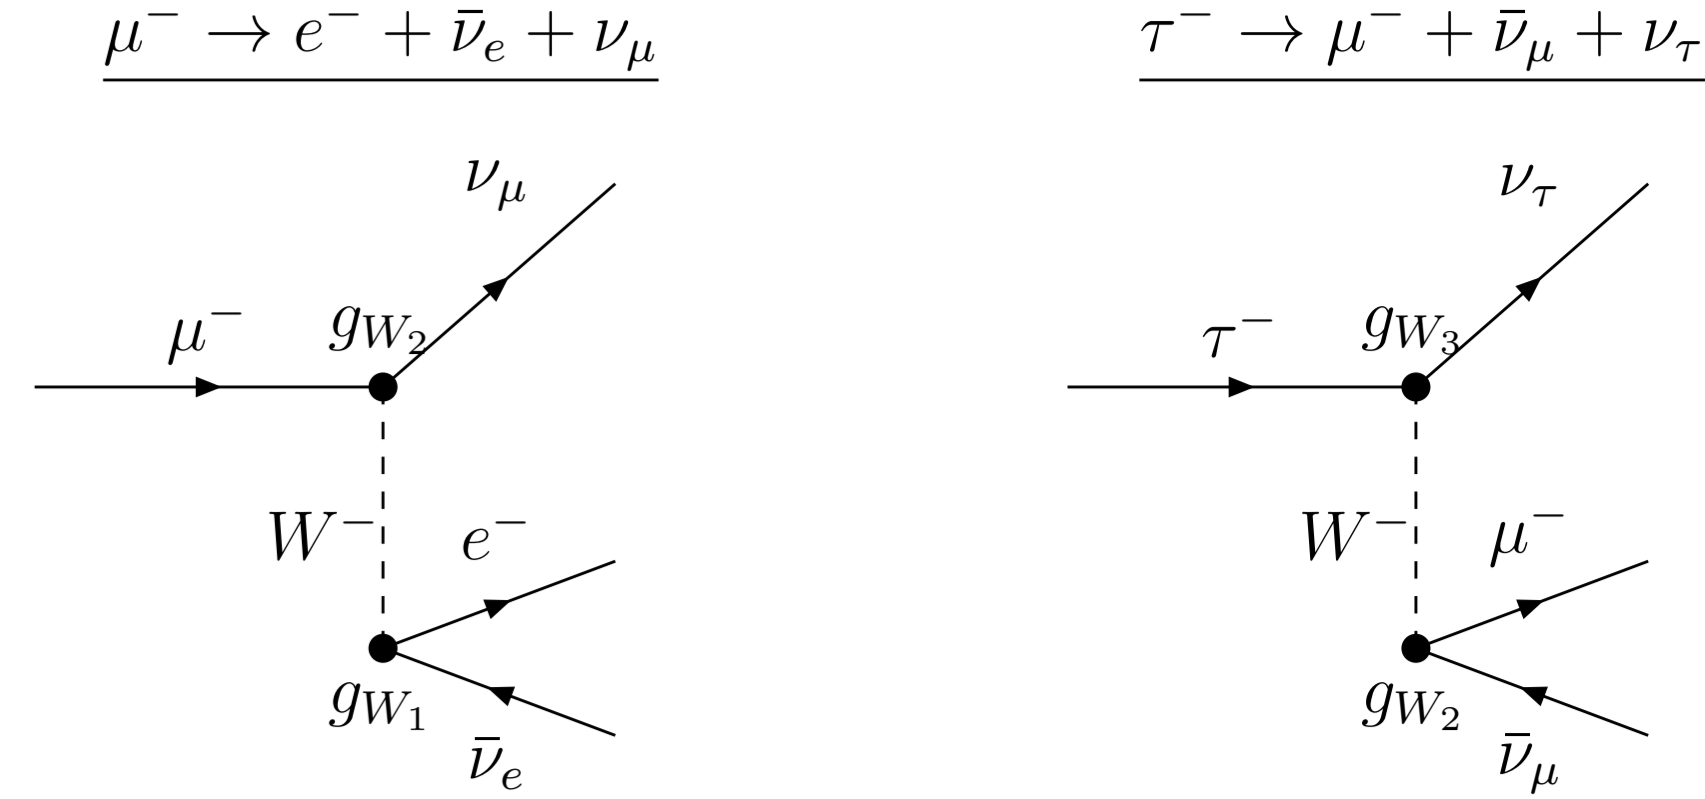
\includegraphics[width=0.75\textwidth]{imagenes/tema2/T2_4_a.png}
    \caption{Diagramas de Feynman para las desintegraciones débiles puramente leptónicas del muón ($\mu^- \to e^- \bar{\nu}_e \nu_\mu$) y del tau ($\tau^- \to \mu^- \bar{\nu}_\mu \nu_\tau$) mediante el intercambio de un bosón $W^-$, con constantes de acoplamiento $g_{W_1}, g_{W_2}, g_{W_3}$ en los vértices.}
    \label{fig:universalidad_debil}
\end{figure}

Para analizar esta cuestión, formulamos la hipótesis de universalidad de los acoplamientos débiles:
\begin{equation}
    g_{W_1} = g_{W_2} = g_{W_3} = g_W
\end{equation}

Para contrastar experimentalmente esta hipótesis, analizamos las anchuras y tiempos de desintegración de los leptones cargados de las tres generaciones:
\begin{itemize}
    \item \textbf{Electrón ($e^-$):} Es una partícula completamente estable ($\tau_e > 6.6 \times 10^{28}\text{ años}$), pues al ser el leptón cargado más ligero, la conservación estricta de la carga eléctrica y del número leptónico electrónico impide cualquier canal de desintegración.
    \item \textbf{Muón ($\mu^-$):} Posee una masa $m_\mu c^2 = 105.658\text{ MeV}$ y un tiempo de vida media $\tau_\mu = 2.197 \times 10^{-6}\text{ s}$. Se desintegra de forma prácticamente exclusiva a través del canal leptónico ($BR = 1$):
    \begin{equation}
        \mu^- \to e^- + \bar{\nu}_e + \nu_\mu
    \end{equation}
    \item \textbf{Tau ($\tau^-$):} Posee una masa $m_\tau c^2 = 1776.93\text{ MeV}$ y un tiempo de vida media $\tau_\tau = 2.903 \times 10^{-13}\text{ s}$. Entre sus diversos canales de desintegración, los dos modos puramente leptónicos principales son:
    \begin{align}
        \tau^- &\to e^- + \bar{\nu}_e + \nu_\tau \quad (BR = 0.1782) \\
        \tau^- &\to \mu^- + \bar{\nu}_\mu + \nu_\tau \quad (BR = 0.1739)
    \end{align}
\end{itemize}

Comparando las masas de los tres leptones cargados con la masa del electrón ($m_e c^2 = 0.511\text{ MeV}$), se observan los siguientes cocientes característicos:
\begin{equation}
    \frac{m_e}{m_\mu} \sim 5 \times 10^{-3}, \quad \frac{m_e}{m_\tau} \sim 3 \times 10^{-4}, \quad \frac{m_\mu}{m_\tau} \sim 6 \times 10^{-2}
\end{equation}

\subsubsection{Estimación teórica de las anchuras de desintegración}

A continuación realizamos una estimación teórica de las anchuras de desintegración del muón y del tau bajo la hipótesis de que la carga débil es universal para las tres generaciones, coincidiendo con la constante de acoplamiento deducida de la desintegración $\beta$ del neutrón libre:
\begin{equation}
    n \to p + e^- + \bar{\nu}_e
\end{equation}

Con una precisión de segundo orden, podemos despreciar las masas de las partículas producidas en el estado final ($m_e, m_\mu \ll m_\tau$). En esta aproximación, el volumen del espacio de fases disponible para un decaimiento de tres cuerpos escala como la quinta potencia de la energía disponible en el centro de masas, $E_0^5 \approx (m_i c^2)^5$, donde $m_i$ representa la masa del leptón inicial.

Todas las desintegraciones débiles nucleares y leptónicas a baja energía pueden expresarse en función de la constante de Fermi $G_F$:
\begin{equation}
    G_F = 8.96 \times 10^{-5}\text{ MeV}\cdot\text{fm}^3 \implies \frac{G_F}{(\hbar c)^3} = 1.166 \times 10^{-5}\text{ GeV}^{-2}
\end{equation}

Bajo la hipótesis de universalidad de la interacción débil entre generaciones leptónicas ($g_{W_1} = g_{W_2} = g_{W_3} = g_W$), se obtienen las siguientes expresiones para las anchuras de desintegración parciales:
\begin{align}
    \Gamma(\mu^- \to e^- + \bar{\nu}_e + \nu_\mu) &= K \left[ \frac{G_F}{(\hbar c)^3} \right]^2 m_\mu^5 \\
    \Gamma(\tau^- \to e^- + \bar{\nu}_e + \nu_\tau) &= K \left[ \frac{G_F}{(\hbar c)^3} \right]^2 m_\tau^5 \\
    \Gamma(\tau^- \to \mu^- + \bar{\nu}_\mu + \nu_\tau) &= K \left[ \frac{G_F}{(\hbar c)^3} \right]^2 m_\tau^5
\end{align}
donde $K = \frac{G_F^2}{192\pi^3}$ representa una constante cinemática proveniente de la integración del elemento de matriz sobre el espacio de fases tridimensional de las partículas finales.

\subsubsection*{Igualdad de las anchuras leptónicas del tau}

Una primera conclusión inmediata de la hipótesis de universalidad es la predicción de la igualdad estricta entre las anchuras de desintegración parciales leptónicas del leptón tau:
\begin{equation}
    \Gamma(\tau^- \to e^- + \bar{\nu}_e + \nu_\tau) = \Gamma(\tau^- \to \mu^- + \bar{\nu}_\mu + \nu_\tau)
\end{equation}

Experimentalmente, las razones de ramificación medidas son:
\begin{equation}
    BR(\tau^- \to e^- + \bar{\nu}_e + \nu_\tau) = 0.1782, \quad BR(\tau^- \to \mu^- + \bar{\nu}_\mu + \nu_\tau) = 0.1739
\end{equation}
lo cual verifica la predicción teórica de igualdad dentro de la precisión experimental disponible. La pequeña diferencia relativa (inferior al $2.5\%$) se explica mediante correcciones de espacio de fases asociadas a la masa no nula del muón en el estado final.

\newpage
\subsubsection*{Verificación experimental del cociente de vidas medias}

Para realizar un contraste cuantitativo riguroso, calculamos el cociente entre las vidas medias del tau y del muón utilizando la hipótesis de universalidad. Partimos de las relaciones generales entre la anchura parcial $\Gamma_i$, la relación de ramificación $BR_i$ y la vida media total $\tau$:
\begin{equation}
    \Gamma_i = BR_i \cdot \Gamma = BR_i \frac{\hbar}{\tau} \implies \tau = \frac{BR_i \, \hbar}{\Gamma_i}
\end{equation}

Por tanto, el cociente entre las vidas medias del tau y del muón se expresa a través del canal de desintegración electrónico como:
\begin{equation}
    \frac{\tau_\tau}{\tau_\mu} = \frac{BR(\tau^- \to e^- + \bar{\nu}_e + \nu_\tau)}{BR(\mu^- \to e^- + \bar{\nu}_e + \nu_\mu)} \cdot \frac{\Gamma(\mu^- \to e^- + \bar{\nu}_e + \nu_\mu)}{\Gamma(\tau^- \to e^- + \bar{\nu}_e + \nu_\tau)}
\end{equation}

Sustituyendo las expresiones teóricas obtenidas para las anchuras en función de la quinta potencia de las masas:
\begin{equation}
    \left. \frac{\tau_\tau}{\tau_\mu} \right|_{\text{Teó}} = \frac{BR(\tau^- \to e^- + \bar{\nu}_e + \nu_\tau)}{1} \cdot \frac{K \left[ \frac{G_F}{(\hbar c)^3} \right]^2 m_\mu^5}{K \left[ \frac{G_F}{(\hbar c)^3} \right]^2 m_\tau^5} = BR(\tau^- \to e^- + \bar{\nu}_e + \nu_\tau) \cdot \left( \frac{m_\mu}{m_\tau} \right)^5
\end{equation}

Sustituyendo los valores numéricos experimentales de las masas ($m_\mu c^2 = 105.658\text{ MeV}$, $m_\tau c^2 = 1776.93\text{ MeV}$) y de la razón de ramificación ($BR = 0.1782$):
\begin{equation}
    \left. \frac{\tau_\tau}{\tau_\mu} \right|_{\text{Teó}} = 0.1782 \times \left( \frac{105.658\text{ MeV}}{1776.93\text{ MeV}} \right)^5 = 0.1782 \times (0.059461)^5 \approx 1.325 \times 10^{-7}
\end{equation}

Comparamos este resultado con el valor experimental directo obtenido a partir de las vidas medias de ambas partículas ($\tau_\mu = 2.19698 \times 10^{-6}\text{ s}$ y $\tau_\tau = 2.903 \times 10^{-13}\text{ s}$):
\begin{equation}
    \left. \frac{\tau_\tau}{\tau_\mu} \right|_{\text{Exp}} = \frac{2.903 \times 10^{-13}\text{ s}}{2.19698 \times 10^{-6}\text{ s}} \approx 1.321 \times 10^{-7}
\end{equation}

El excelente acuerdo entre la predicción teórica ($1.325 \times 10^{-7}$) y el valor experimental ($1.321 \times 10^{-7}$) constituye una prueba concluyente de la \textbf{universalidad de la interacción débil} para los leptones de las tres generaciones del Modelo Estándar.

\newpage
\subsection{5 - Unificación}

La amplitud de dispersión entre dos partículas con carga $g$, mediada por el intercambio de un bosón gauge vectorial de masa $m$, viene dada en el espacio de momentos por:
\begin{equation}
    A(\vec{q}) = 4\pi \, \alpha_g \frac{(\hbar c)^3}{m^2 c^4 + q^2 c^2}
\end{equation}
donde $\alpha_g = \frac{g^2}{4\pi \varepsilon_0 \hbar c}$ representa la constante de acoplamiento adimensional e $i\vec{q}$ la transferencia de momento espacial.

En el límite en el que el bosón mediador es muy masivo en comparación con el momento transferido en el proceso ($m c^2 \gg q c$), el denominador puede aproximarse por la masa del bosón en reposo, y la amplitud se simplifica a:
\begin{equation}
    A(\vec{q}) \approx 4\pi \, \alpha_g \frac{(\hbar c)^3}{m^2 c^4} \equiv \text{constante efectiva}
\end{equation}

Este es precisamente el caso de la interacción débil a baja energía en procesos nucleares, donde las transferencias de energía o momento son del orden $Q \sim 2\text{ MeV}$, mientras que las masas de los bosones vectoriales mediadores $W^\pm$ y $Z^0$ son enormes ($m_{W^\pm} c^2 \approx 80.4\text{ GeV}$ y $m_{Z^0} c^2 \approx 91.2\text{ GeV}$).

Dicha constante efectiva rige la intensidad de los procesos débiles a baja energía y se identifica directamente con la constante de Fermi $G_F$:
\begin{equation}
    4\pi \, \alpha_W \frac{(\hbar c)^3}{m_W^2 c^4} = G_F
\end{equation}
donde dimensionalmente $\left[ \frac{G_F}{(\hbar c)^3} \right] \equiv E^{-2}$, alcanzando el valor experimental característico:
\begin{equation}
    \frac{G_F}{(\hbar c)^3} = 1.166 \times 10^{-5}\text{ GeV}^{-2}
\end{equation}

Si suponemos la hipótesis de unificación de que la constante de acoplamiento débil intrínseca $\alpha_W$ es del mismo orden de magnitud que la constante de estructura fina electromagnética ($\alpha_W \approx \alpha \approx 1/137$), despejamos la masa necesaria para el bosón $W$:
\begin{equation}
    m_W c^2 = \sqrt{\frac{4\pi \alpha_W}{\frac{G_F}{(\hbar c)^3}}} \approx \sqrt{\frac{4\pi \times (1/137)}{1.166 \times 10^{-5}\text{ GeV}^{-2}}} \approx 88.7\text{ GeV}
\end{equation}

Este resultado anticipó con precisión la escala de masas de los bosones $W^\pm$ y $Z^0$ antes de su descubrimiento experimental en el CERN, demostrando que la aparente debilidad de la fuerza débil a bajas energías no proviene de una carga pequeña ($\alpha_W \sim \alpha$), sino del confinamiento de la interacción a corto alcance producido por la \textbf{enorme masa de los bosones mediadores}.

En las secciones precedentes se ha caracterizado cada interacción fundamental mediante su constante de acoplamiento adimensional en el régimen de bajas energías, obteniéndose valores aparentemente muy dispares:
\[
\begin{array}{l}
    \displaystyle \alpha_s \sim 1 \quad \text{(interacción fuerte)}, \\[4pt]
    \displaystyle \alpha \approx \frac{1}{137} \sim 10^{-2} \quad \text{(interacción electromagnética)}, \\[4pt]
    \displaystyle \alpha_W \sim 10^{-7} \quad \text{(interacción débil)}
\end{array}
\]

En esta sección se aborda la unificación de la interacción electromagnética y la interacción débil en el marco del \textbf{Modelo Electrodébil}, demostrando que la aparente debilidad de la fuerza débil a baja energía no constituye una propiedad intrínseca de sus vértices de acoplamiento, sino una consecuencia directa del mecanismo de propagación mediado por bosones vectoriales masivos.

\subsubsection{Amplitud de dispersión y régimen de bajas energías}

En Teoría Cuántica de Campos, la dispersión elástica entre dos partículas con carga genérica $g$, mediada por la emisión y absorción de un bosón gauge masivo de masa $m$, viene descrita en el espacio de momentos en el límite estático por la amplitud $A(\vec{q})$:
\begin{equation}
    A(\vec{q}) = 4\pi \, \alpha_g \frac{(\hbar c)^3}{m^2 c^4 + q^2 c^2}
\end{equation}
donde $\alpha_g = \frac{g^2}{4\pi \varepsilon_0 \hbar c}$ representa la constante de acoplamiento adimensional del vértice e $i\vec{q}$ denota el vector de transferencia de momento tridimensional entre las partículas ($q = |\vec{q}|$).

\subsubsection*{Límite estático de contacto}

En los procesos nucleares y leptónicos a baja energía (tales como la desintegración $\beta$ del neutrón o el decaimiento de mesones y muones), la energía típica liberada en la reacción es de orden $Q \sim 2 \text{ MeV} - 100 \text{ MeV}$. Por ende, el momento transferido satisface la condición de supresión $qc \sim Q \ll mc^2$ frente a la masa de los bosones intermediarios ($m_{W^\pm, Z^0} \sim 80 - 90 \text{ GeV}/c^2$).

Factorizando la masa del mediador en el denominador de la amplitud:
\begin{equation}
    A(\vec{q}) = 4\pi \, \alpha_g \frac{(\hbar c)^3}{m^2 c^4 \left( 1 + \frac{q^2 c^2}{m^2 c^4} \right)} = 4\pi \, \alpha_g \frac{(\hbar c)^3}{m^2 c^4} \left( 1 - \frac{q^2 c^2}{m^2 c^4} + \mathcal{O}\left( \frac{q^4 c^4}{m^4 c^8} \right) \right)
\end{equation}

Al tomar el límite $qc \ll mc^2$, la dependencia en el momento transferido $q$ desaparece, y la amplitud se simplifica a una constante efectiva independiente de la dinámica espacial:
\begin{equation}
    A(\vec{q}) \approx 4\pi \, \alpha_g \frac{(\hbar c)^3}{m^2 c^4} \equiv \text{constante efectiva}
\end{equation}

En el espacio de posiciones, la transformada de Fourier inversa de una constante en el espacio de momentos conduce de forma exacta a un potencial de contacto puntual de tipo delta de Dirac:
\begin{equation}
    V(\vec{r}) = \int \frac{d^3q}{(2\pi\hbar)^3} A(\vec{q}) e^{-i \vec{q} \cdot \vec{r} / \hbar} = \left( 4\pi \, \alpha_g \frac{(\hbar c)^3}{m^2 c^4} \right) \delta^{(3)}(\vec{r})
\end{equation}

Esta constante efectiva rige la intensidad de los procesos débiles a baja energía y se identifica directamente con la \textbf{constante de Fermi} $G_F$:
\begin{equation}
    4\pi \, \alpha_W \frac{(\hbar c)^3}{m^2 c^4} = G_F
\end{equation}
donde las dimensiones de la constante de Fermi normalizada vienen dadas por:
\begin{equation}
    \left[ \frac{G_F}{(\hbar c)^3} \right] \equiv E^{-2} \quad \implies \quad \frac{G_F}{(\hbar c)^3} = 1.166 \times 10^{-5} \text{ GeV}^{-2}
\end{equation}

\newpage
\subsubsection{Inconsistencia de la estimación naïve de la masa del mediador}

Si intentamos despejar la masa del bosón mediador $mc^2$ utilizando directamente el valor de la constante de acoplamiento débil adimensional hallada previamente mediante la tasa de desintegración ($\alpha_W \sim 10^{-7}$), se obtiene:
\begin{equation}
    mc^2 = \sqrt{\frac{4\pi \alpha_W}{\frac{G_F}{(\hbar c)^3}}} = \sqrt{\frac{4\pi \times 10^{-7}}{1.166 \times 10^{-5} \text{ GeV}^{-2}}} \approx 0.328 \text{ GeV}
\end{equation}

\begin{observacion}[Inconsistencia física del modelo de acoplamiento débil puro]
El valor predicho $mc^2 \approx 0.328 \text{ GeV}$ resulta completamente inconsistente con la física observada por dos razones fundamentales:
\begin{enumerate}
    \item Implicaría que la masa del bosón mediador es del mismo orden de magnitud que la escala de momentos involucrada en la física hadrónica ($\sim 300 \text{ MeV}$), lo que contradiría el carácter de muy corto alcance ($\sim 10^{-18} \text{ m}$) de la interacción débil.
    \item Predeciría la existencia de estados ligados débiles estables en la naturaleza, los cuales no han sido detectados en ningún experimento.
\end{enumerate}
\end{observacion}

\newpage
\subsubsection{El Modelo Electrodébil (Glashow-Salam-Weinberg)}

La raíz del problema anterior reside en haber interpretado la constante reducida $\alpha_W \sim 10^{-7}$ como el acoplamiento fundamental del vértice. En la década de 1960, S. L. Glashow, A. Salam y S. Weinberg formularon el \textbf{Modelo Electrodébil}, que unifica las fuerzas electromagnética y débil en un marco de simetría de calibre basada en el grupo de Lie $SU(2)_L \times U(1)_Y$.

La teoría se fundamenta en dos constantes de acoplamiento gauge primarias:
\begin{itemize}
    \item $g$: constante de acoplamiento asociada al isospín débil $SU(2)_L$.
    \item $g'$: constante de acoplamiento asociada a la hipercarga débil $U(1)_Y$.
\end{itemize}

Los campos físicos observables (el fotón no masivo $\gamma$, los bosones cargados masivos $W^\pm$ y el bosón neutro masivo $Z^0$) se obtienen como combinaciones lineales de los campos de calibre originales tras el mecanismo de ruptura espontánea de simetría (mecanismo de Higgs). 

En particular, la carga eléctrica fundamental $e$ de la interacción electromagnética no es un parámetro independiente, sino que se relaciona con las cargas primarias a través del \textbf{ángulo de mezcla débil o ángulo de Weinberg} $\theta_W$:
\begin{equation}
    e = g \sin\theta_W = g' \cos\theta_W
\end{equation}

A partir de las mediciones experimentales de precisión en colisionadores:
\begin{equation}
    \sin^2\theta_W \approx 0.231 \implies \sin\theta_W \approx 0.48, \quad \cos\theta_W \approx 0.88
\end{equation}

Puesto que $\sin\theta_W \sim \mathcal{O}(1)$, se deduce inmediatamente que las constantes de acoplamiento fundamentales $g$, $g'$ y $e$ son del mismo orden de magnitud. Expresado en términos de constantes de estructura adimensionales:
\begin{equation}
    \alpha_g = \frac{g^2}{4\pi \hbar c} \sim \alpha = \frac{e^2}{4\pi \varepsilon_0 \hbar c} \approx \frac{1}{137}
\end{equation}

Es decir, la intensidad intrínseca de la interacción débil en los vértices de acoplamiento es **idéntica en orden de magnitud a la intensidad de la interacción electromagnética**.

\newpage
\subsubsection{Predicción unificada de la masa de los bosones $W^\pm$ y $Z^0$}

Sustituyendo el acoplamiento unificado $\alpha_g \sim \alpha \approx 1/137$ en la relación de la constante de Fermi, recalculamos la escala de masa de los bosones intermediarios:
\begin{align}
    mc^2 &\sim \sqrt{\frac{4\pi \alpha}{\frac{G_F}{(\hbar c)^3}}} = \sqrt{\frac{4\pi \times \left( \frac{1}{137.036} \right)}{1.16638 \times 10^{-5} \text{ GeV}^{-2}}} \nonumber \\
    &= \sqrt{\frac{0.091703}{1.16638 \times 10^{-5} \text{ GeV}^{-2}}} = \sqrt{7862.2 \text{ GeV}^2} \approx 88.68 \text{ GeV}
\end{align}

Este resultado teórico se encuentra en un acuerdo excelente con las masas medidas experimentalmente para los bosones vectoriales de la interacción débil:
\begin{equation}
    m_{W^\pm} = 80.37 \text{ GeV}/c^2, \quad m_{Z^0} = 91.188 \text{ GeV}/c^2
\end{equation}

\newpage
\subsubsection{Origen de la aparente debilidad: Efecto del propagador}

¿Por qué en los experimentos de baja energía dedujimos inicialmente una constante efectiva $\alpha_W \sim 10^{-7} \ll \alpha$?

La razón radica en que la amplitud de cualquier proceso microscópico es el producto del acoplamiento en los vértices por el **propagador** del bosón mediador. Trabajando en unidades naturales ($\hbar = c = 1$):

\begin{enumerate}
    \item \textbf{Interacción electromagnética:} Mediada por el fotón sin masa ($m_\gamma = 0$). La amplitud de dispersión viene modulada por el propagador fotónico $1/q^2$:
    \begin{equation}
        A_{\text{EM}}(q) \propto \sqrt{\alpha} \cdot \left( \frac{1}{q^2} \right) \cdot \sqrt{\alpha} = \frac{\alpha}{q^2}
    \end{equation}
    
    \item \textbf{Interacción débil:} Mediada por los bosones masivos $W^\pm$ o $Z^0$ ($m \neq 0$). La amplitud exacta satisface:
    \begin{equation}
        A_W(q) \propto \sqrt{\alpha} \cdot \left( \frac{1}{q^2 + m^2} \right) \cdot \sqrt{\alpha} = \frac{\alpha}{q^2 + m^2}
    \end{equation}
\end{enumerate}

En el régimen de bajas energías ($q \ll m$), el propagador masivo se contrae a $1/(q^2 + m^2) \approx 1/m^2$, resultando:
\begin{equation}
    A_W \propto \frac{\alpha}{m^2} = \frac{\alpha}{q^2} \left( \frac{q^2}{m^2} \right)
\end{equation}

Por lo tanto, la constante efectiva $\alpha_W$ hallada previamente no es más que el acoplamiento electromagnético suprimido por el factor adimensional $(q/m)^2$:
\begin{equation}
    \alpha_W \sim \alpha \left( \frac{q^2}{m^2} \right) \sim 10^{-2} \times \left( \frac{10^{-3} \text{ GeV}}{100 \text{ GeV}} \right)^2 \sim 10^{-2} \times 10^{-10} \sim 10^{-12} - 10^{-7}
\end{equation}

\begin{concepto}[Dominancia del propagador vs. estructura de vértices]
La intensidad global de una interacción no está determinada únicamente por los vértices de acoplamiento, sino por la combinación del vértice y el propagador del bosón mediador:
\begin{itemize}
    \item **A bajas energías ($q \ll m$):** La física está completamente dominada por el propagador masivo, el cual induce una supresión drástica de la amplitud por un factor $1/m^2$. Esto da la falsa apariencia de que la fuerza débil es intrínsecamente "débil".
    \item **A altas energías ($q \gg m$):** La masa del mediador pasa a ser despreciable frente a la transferencia de momento ($q^2 + m^2 \approx q^2$). El propagador débil recupera la forma $1/q^2$ y la amplitud débil alcanza exactamente la misma magnitud que la interacción electromagnética, manifestándose la simetría electrodébil unificada.
\end{itemize}
\end{concepto}

\begin{figure}[htbp]
    \centering
    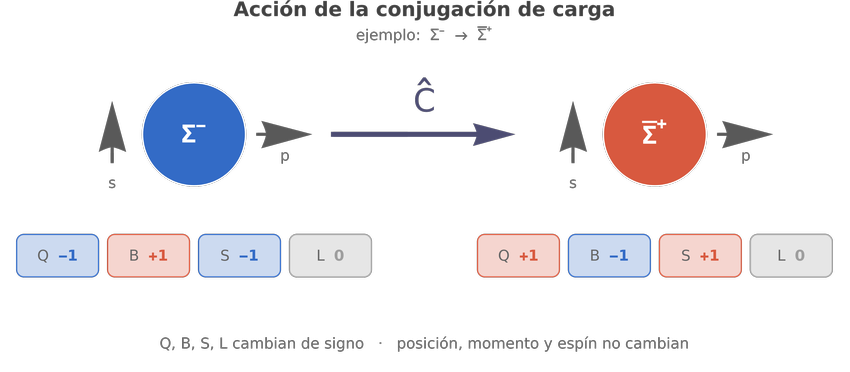
\includegraphics[width=0.85\textwidth]{imagenes/tema2/T2_5_a.png}
\end{figure}

\newpage
\section{Paridad}

La \textbf{paridad} es una simetría discreta que corresponde a la inversión espacial de las coordenadas cartesianas:
\begin{equation}
    \vec{r} \longrightarrow -\vec{r}
\end{equation}

En mecánica cuántica, la paridad se asocia a un operador cuántico $\hat{P}$. Sus propiedades algebraicas fundamentales son las siguientes:
\begin{itemize}
    \item \textbf{Hermiticidad:} Como la paridad corresponde a una cantidad físicamente observable, el operador $\hat{P}$ es hermítico:
    \begin{equation}
        \hat{P}^\dagger = \hat{P}
    \end{equation}
    \item \textbf{Involución:} Aplicar dos inversiones espaciales consecutivas devuelve el sistema a su estado original:
    \begin{equation}
        \hat{P}^2 = \mathbb{I} \implies \hat{P}^{-1} = \hat{P}
    \end{equation}
    \item \textbf{Unitariedad:} Combinando la hermiticidad y la involución se deduce que $\hat{P}^{-1} = \hat{P}^\dagger$, por lo que $\hat{P}$ es un operador unitario.
    \item \textbf{Autovalores:} Si $|\psi\rangle$ es un autoestado de paridad con autovalor $P$:
    \begin{equation}
        \hat{P}^2 |\psi\rangle = P^2 |\psi\rangle = |\psi\rangle \implies P^2 = 1 \implies P = \pm 1
    \end{equation}
    Por tanto, los únicos autovalores posibles de la paridad son $P = +1$ (paridad par o positiva) y $P = -1$ (paridad impar o negativa).
\end{itemize}

La paridad es una simetría exacta en las interacciones fuerte y electromagnética ($[\hat{P}, H] = 0$), pero se viola explícitamente en la interacción débil.

\subsection{Clasificación de estados y el fotón}

Para caracterizar el estado cuántico de una partícula o campo, se especifica su momento angular total $J$ y su paridad $P$, denotado como $J^P$. En el caso de los bosones, la nomenclatura sigue el comportamiento de transformación de tensores bajo paridad:
\begin{itemize}
    \item \textbf{Vector polar:} Cambia de signo bajo paridad, $\vec{r} \to -\vec{r}$ ($J^P = 1^-$).
    \item \textbf{Vector axial (pseudovector):} No cambia de signo bajo paridad, como el momento angular $\vec{L} = \vec{r} \times \vec{p} \to (-\vec{r}) \times (-\vec{p}) = \vec{L}$ ($J^P = 1^+$).
    \item \textbf{Escalar:} Invariante bajo paridad, $a = \vec{\alpha}_1 \cdot \vec{\alpha}_2 \to a$ ($J^P = 0^+$).
    \item \textbf{Pseudoescalar:} Cambia de signo bajo paridad, $b = \vec{p}_1 \cdot \vec{\alpha}_1 \to (- \vec{p}_1) \cdot \vec{\alpha}_1 = -b$ ($J^P = 0^-$).
\end{itemize}

En teoría clásica, el campo electromagnético viene descrito por el potencial vectorial $\vec{A}(\vec{r}, t)$, el cual satisface en el vacío la ecuación de ondas:
\begin{equation}
    \nabla^2 \vec{A}(\vec{r},t) - \frac{1}{c^2}\frac{\partial^2 \vec{A}(\vec{r},t)}{\partial t^2} = 0
\end{equation}
En mecánica cuántica, el fotón ($\gamma$) es el cuanto asociado al campo vectorial electromagnético $\vec{A}(\vec{r},t)$. Como $\vec{A}$ transforma como un vector polar ($\vec{A} \to -\vec{A}$), el fotón es una partícula de espín $J_\gamma = 1$ y paridad negativa, caracterizado por $J_\gamma^P = 1^-$.

\subsection{Paridad de un sistema físico}

\subsubsection{Dos partículas}

Consideremos dos partículas que interaccionan mediante un potencial central $V(\vec{r}_{12}) = V(r)$, donde $\vec{r} = \vec{r}_1 - \vec{r}_2$. La función de onda espacial del estado de movimiento relativo se escribe como:
\begin{equation}
    \Psi_{nlm_l}(\vec{r}) = R_{nl}(r) Y_{lm_l}(\theta, \varphi)
\end{equation}

Bajo una transformación de paridad $\vec{r} \to -\vec{r}$, las coordenadas esféricas se transforman según:
\begin{equation}
    r \to r, \quad \theta \to \pi - \theta, \quad \varphi \to \pi + \varphi
\end{equation}

La parte radial permanece inalterada ($R_{nl}(r) \to R_{nl}(r)$), mientras que los armónicos esféricos satisfacen la relación de simetría:
\begin{equation}
    Y_{lm_l}(\pi - \theta, \pi + \varphi) = (-1)^l Y_{lm_l}(\theta, \varphi)
\end{equation}

Por lo tanto, la acción del operador paridad sobre la función de onda espacial resulta:
\begin{equation}
    \hat{P} \Psi_{nlm_l}(\vec{r}) = (-1)^l \Psi_{nlm_l}(\vec{r})
\end{equation}

Así, la paridad orbital de un sistema de dos partículas viene dada exclusivamente por $(-1)^l$, donde $l$ es el momento angular orbital relativo. En el caso de partículas idénticas, esta paridad coincide con la simetría de intercambio de la parte espacial. No obstante, es fundamental recalcar que la paridad (inversión espacial de coordenadas) y la simetría bajo intercambio de partículas son operaciones conceptualmente distintas.

\subsubsection{Varias partículas}

Para un sistema de $N$ partículas con un potencial central separable en términos de $N-1$ coordenadas relativas de Jacobi $\vec{\lambda}_k$:
\begin{equation}
    V(\vec{r}_1, \dots, \vec{r}_N) = \sum_{k=1}^{N-1} V(\vec{\lambda}_k) \implies \Psi(\vec{r}_1, \dots, \vec{r}_N) = \prod_{k=1}^{N-1} \psi_{n_k l_k m_{l_k}}(\vec{\lambda}_k)
\end{equation}

Bajo inversión espacial, cada coordenada de Jacobi invierte su signo ($\vec{\lambda}_k \to -\vec{\lambda}_k$), aportando un factor $(-1)^{l_k}$. En consecuencia, la paridad espacial total del sistema es:
\begin{equation}
    \hat{P} \Psi(\vec{r}_1, \dots, \vec{r}_N) = \prod_{k=1}^{N-1} \hat{P} \psi_{n_k l_k m_{l_k}}(\vec{\lambda}_k) = (-1)^{\sum_{k=1}^{N-1} l_k} \Psi(\vec{r}_1, \dots, \vec{r}_N)
\end{equation}

Debido al acoplamiento vectorial de momentos angulares (series de Clebsch-Gordan), la paridad total depende de la \textbf{suma algebraica} de los momentos angulares relativos $\sum l_k$, mientras que el momento angular orbital total $L$ se obtiene mediante la \textbf{suma vectorial} de los mismos. Por ello, en general no existe una relación directa entre la paridad espacial y $(-1)^L$.

Un caso particular de interés ocurre para un sistema de tres partículas con momento angular orbital total $L = 0$. La condición de acoplamiento vectorial exige que los momentos angulares parciales satisfagan $l_{12} = l_{(12)3}$. De este modo, la suma algebraica es:
\begin{equation}
    l_{12} + l_{(12)3} = 2 l_{12} \quad \text{(necesariamente un número par)}
\end{equation}
por lo que la paridad orbital total $(-1)^{2 l_{12}} = +1$ es estrictamente positiva.

\subsection{Paridad intrínseca}

Consideremos un estado de partícula libre $a$ con momento $\vec{p}$, descrito por una función de onda plana:
\begin{equation}
    \Psi_{\vec{p}}^a(\vec{r}, t) = N e^{-i(\vec{p}\cdot\vec{r} - Et)/\hbar}
\end{equation}
Al aplicar el operador de paridad espacial:
\begin{equation}
    \hat{P} \Psi_{\vec{p}}^a(\vec{r}, t) = P_a \Psi_{\vec{p}}^a(-\vec{r}, t) = P_a \Psi_{-\vec{p}}^a(\vec{r}, t)
\end{equation}

En el sistema en reposo de la partícula ($\vec{p} = \vec{0}$), esta transformación se convierte en una ecuación de autovalores:
\begin{equation}
    \hat{P} \Psi_{\vec{0}}^a(\vec{r}, t) = P_a \Psi_{\vec{0}}^a(\vec{r}, t)
\end{equation}
donde $P_a = \pm 1$ se define como la \textbf{paridad intrínseca} de la partícula.

\paragraph{Necesidad de la paridad intrínseca en mecánica cuántica relativista:}
En mecánica cuántica no relativista, el número de partículas se conserva y no existen antipartículas, por lo que las fases relativas entre distintos tipos de partículas no influyen en los observables físicos. En cambio, en mecánica cuántica relativista (desprimiendo ecuaciones como la de Dirac), los campos contienen grados de libertad de partículas y antipartículas que pueden crearse y aniquilarse. La invariance de Dirac bajo paridad exige que un fermión de espín $1/2$ y su correspondiente antifermión posean \textbf{paridades intrínsecas opuestas}:
\begin{equation}
    P_{\text{fermión}} P_{\text{antifermión}} = -1
\end{equation}
mientras que para bosones y antibosones la paridad intrínseca es la misma ($P_{\text{bosón}} P_{\text{antibosón}} = +1$).

\paragraph{Determinación experimental mediante el positronio ($e^+ e^-$):}
El positronio es un estado ligado electrón-positrón. Su estado fundamental se encuentra en onda $S$ ($L_{e^-e^+} = 0$). Presenta dos configuraciones de espín:
\begin{itemize}
    \item \textbf{Ortopositronio} ($^3S_1$): Estado triplete ($S = 1$).
    \item \textbf{Parapositronio} ($^1S_0$): Estado singlete ($S = 0$), correspondiente al estado fundamental de menor energía.
\end{itemize}

Consideremos el canal de desintegración electromagnética del parapositronio en dos fotones:
\begin{equation}
    e^+ + e^- \, [^1S_0 (L_{e^-e^+}=0, S_{e^-e^+}=0)] \longrightarrow \gamma + \gamma
\end{equation}

Por conservación de la paridad en la interacción electromagnética:
\begin{equation}
    P_i = P_{e^+} P_{e^-} (-1)^{L_{e^-e^+}} = P_{e^+} P_{e^-} (-1)^0 = P_{e^+} P_{e^-}
\end{equation}
\begin{equation}
    P_f = P(\gamma \gamma) \implies P_{e^+} P_{e^-} = P(\gamma \gamma)
\end{equation}

Para determinar $P(\gamma\gamma)$, analizamos las propiedades cinemáticas del estado final de dos fotones. Como el estado inicial tiene momento angular total $J_i = 0$, la conservación del momento angular exige $J_f = 0$.

En el sistema centro de masas, los momentos de los dos fotones son opuestos ($\vec{k}_1 = \vec{k}$, $\vec{k}_2 = -\vec{k}$), y sus vectores de polarización transversal son $\vec{\epsilon}_1$ y $\vec{\epsilon}_2$. Para un estado escalar de dos fotones con $J=0$, existen únicamente dos combinaciones posibles de polarización:
\begin{enumerate}
    \item \textbf{Estado Escalar ($J^P = 0^+$):} $\vec{\epsilon}_1 \cdot \vec{\epsilon}_2$ (polarizaciones paralelas).
    \item \textbf{Estado Pseudoescalar ($J^P = 0^-$):} $(\vec{\epsilon}_1 \times \vec{\epsilon}_2) \cdot \vec{k}$ (polarizaciones perpendiculares).
\end{enumerate}

Bajo una inversión espacial ($\vec{r} \to -\vec{r}$), el momento cambia de signo ($\vec{k} \to -\vec{k}$), mientras que los vectores de polarización (campos eléctricos) invierten su signo ($\vec{\epsilon} \to -\vec{\epsilon}$). Al evaluar la paridad de la combinación pseudoescalar:
\begin{equation}
    \hat{P} \left[ (\vec{\epsilon}_1 \times \vec{\epsilon}_2) \cdot \vec{k} \right] = ((-\vec{\epsilon}_1) \times (-\vec{\epsilon}_2)) \cdot (-\vec{k}) = - (\vec{\epsilon}_1 \times \vec{\epsilon}_2) \cdot \vec{k}
\end{equation}
obtenemos un signo negativo, correspondiente a paridad $P = -1$.

Los experimentos de correlación angular de polarización (Wu y Shaknov, 1950) confirmaron que los fotones emitidos en la desintegración del parapositronio tienen vectores de polarización preferentemente \textbf{perpendiculares}. Esto demuestra que el estado final de dos fotones es un pseudoescalar ($J^P = 0^-$), por lo que $P(\gamma\gamma) = -1$.

En consecuencia, deducimos experimentalmente la relación fundamental:
\begin{equation}
    P_{e^+} P_{e^-} = -1
\end{equation}
demostrando que el electrón y el positrón poseen paridades intrínsecas opuestas, tal y como predice la teoría cuántica relativista de Dirac.
\subsubsection*{Convenio de fases y paridad de sistemas compuestos}

Como se ha demostrado en el marco de la teoría cuántica relativista, no es posible asignar una paridad intrínseca absoluta a un fermión o a su antifermión de manera independiente, sino únicamente definir su paridad relativa:
\begin{equation}
    P_f P_{\bar{f}} = -1
\end{equation}

Para poder construir de forma consistente y unívoca los números cuánticos de paridad en estados ligados e interacciones hadrónicas o nucleares, se fija un convenio internacional de fases para las partículas elementales:
\begin{itemize}
    \item \textbf{Fermiones (partículas):} Se les asigna por convenio paridad intrínseca positiva:
    \begin{equation}
        P_{e^-} = P_{\mu^-} = P_{\tau^-} = P_q = +1
    \end{equation}
    \item \textbf{Antifermiones (antipartículas):} En virtud de la relación $P_f P_{\bar{f}} = -1$, las antipartículas poseen necesariamente paridad negativa:
    \begin{equation}
        P_{e^+} = P_{\mu^+} = P_{\tau^+} = P_{\bar{q}} = -1
    \end{equation}
\end{itemize}

\begin{observacion}[Paridad en neutrinos]
Los neutrinos no poseen una paridad intrínseca bien definida en el Modelo Estándar. Debido a su carácter quiral y a que participan únicamente en corrientes cargadas débiles que violan al máximo la paridad (solo se observan neutrinos levógiros $\nu_L$ y antineutrinos dextrógiros $\bar{\nu}_R$), no es posible asignarles un autovalor de paridad.
\end{observacion}

A partir de este convenio fundamental, se derivan de forma rigurosa las paridades intrínsecas de los sistemas compuestos:

\paragraph{1. Paridad de los mesones ($M = q\bar{q}$):}
Un mesón se compone de un quark ($P_q = +1$) y un antiquark ($P_{\bar{q}} = -1$) ligados con un momento angular orbital relativo $L_{q\bar{q}}$. La paridad total del mesón viene dada por:
\begin{equation}
    P_M = P_q P_{\bar{q}} (-1)^{L_{q\bar{q}}} = (+1)(-1)(-1)^{L_{q\bar{q}}} = (-1)^{L_{q\bar{q}} + 1}
\end{equation}
Para la antipartícula correspondiente $\bar{M} = \bar{q}q$:
\begin{equation}
    P_{\bar{M}} = P_{\bar{q}} P_q (-1)^{L_{q\bar{q}}} = (-1)(+1)(-1)^{L_{q\bar{q}}} = (-1)^{L_{q\bar{q}} + 1} = P_M
\end{equation}
Por consiguiente, para cualquier estado bosónico $b$ y su antibosón $\bar{b}$ se verifica de forma general:
\begin{equation}
    P_b P_{\bar{b}} = +1
\end{equation}

\paragraph{2. Paridad de los bariones ($B = q_1 q_2 q_3$):}
Un barión consta de tres quarks de valencia. Su paridad se obtiene multiplicando las paridades intrínsecas de los tres quarks por los factores espaciales asociados a las dos coordenadas relativas de Jacobi ($L_{q_1 q_2}$ y $L_{(q_1 q_2)q_3}$):
\begin{equation}
    P_B = P_{q_1} P_{q_2} P_{q_3} (-1)^{L_{q_1 q_2} + L_{(q_1 q_2)q_3}} = (+1)^3 (-1)^{L_{q_1 q_2} + L_{(q_1 q_2)q_3}} = (-1)^{L_{q_1 q_2} + L_{(q_1 q_2)q_3}}
\end{equation}
Para el antibarión formado por tres antiquarks ($\bar{B} = \bar{q}_1 \bar{q}_2 \bar{q}_3$):
\begin{equation}
    P_{\bar{B}} = P_{\bar{q}_1} P_{\bar{q}_2} P_{\bar{q}_3} (-1)^{L_{\bar{q}_1 \bar{q}_2} + L_{(\bar{q}_1 \bar{q}_2)\bar{q}_3}} = (-1)^3 (-1)^{L_{q_1 q_2} + L_{(q_1 q_2)q_3}} = -P_B
\end{equation}
se comprueba que para todo sistema fermiónico se satisface de nuevo la regla general:
\begin{equation}
    P_f P_{\bar{f}} = -1
\end{equation}
\newpage
%=============================================================
% Sección 4. Subsección c) PARIDAD DEL FOTÓN 
%=============================================================
\subsection{Paridad del fotón}

Las propiedades del fotón ($\gamma$) se infieren mediante el \textbf{Principio de Correspondencia} de Bohr, el cual exige que las predicciones de la teoría cuántica converjan con las leyes de la electrodinámica clásica de Maxwell en el límite de campos macrorradiativos.

Para determinar la paridad intrínseca del fotón, se analizan las propiedades de simetría de las ecuaciones del campo electromagnético bajo la inversión espacial $\vec{r} \to -\vec{r}$.
\begin{figure}[htbp]
    \centering
    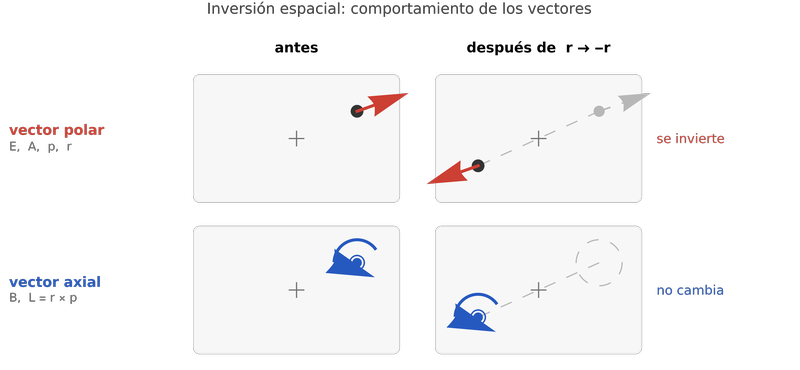
\includegraphics[width=0.95\textwidth]{imagenes/tema2/T2_4_paridad_foton_a.png}
    \caption{Compara qué le pasa a un vector polar ($\vec E,\vec A,\vec p,\vec r$), que se invierte con $\vec r\to-\vec r$, y a uno axial ($\vec B,\vec L$), que conserva su sentido de giro. Es el vocabulario que usas en el texto.}
    \label{fig:T2_4_paridad_foton_a}
\end{figure}

\subsubsection*{1. Comportamiento del campo eléctrico $\vec{E}(\vec{r},t)$ bajo paridad}

Consideremos la Ley de Gauss electromagnética en un medio con densidad de carga $\rho(\vec{r},t)$:
\begin{equation}
    \vec{\nabla} \cdot \vec{E}(\vec{r},t) = \frac{1}{\varepsilon_0} \rho(\vec{r},t)
\end{equation}

Bajo la transformación discreta de paridad $\vec{r} \to -\vec{r}$:
\begin{enumerate}
    \item El operador nabla (derivada espacial) invierte su signo por tratarse de un operador diferencial vectorial:
    \begin{equation}
        \vec{\nabla} = \left( \frac{\partial}{\partial x}, \frac{\partial}{\partial y}, \frac{\partial}{\partial z} \right) \longrightarrow -\vec{\nabla}
    \end{equation}
    \item La densidad de carga escalar $\rho(\vec{r},t)$ satisface:
    \begin{equation}
        \rho(\vec{r},t) \longrightarrow \rho(-\vec{r},t)
    \end{equation}
\end{enumerate}

Para que la Ley de Gauss mantenga la invariancia de forma (simetría espacial) en las nuevas coordenadas invertidas:
\begin{equation}
    (-\vec{\nabla}) \cdot \vec{E}'(-\vec{r},t) = \frac{1}{\varepsilon_0} \rho(-\vec{r},t)
\end{equation}
Comparando esta igualdad con la ecuación original evaluada en el punto $-\vec{r}$, se concluye que el campo eléctrico debe transformar necesariamente como un \textbf{vector polar}:
\begin{equation}
    \vec{E}(\vec{r},t) \longrightarrow -\vec{E}(-\vec{r},t)
\end{equation}

\begin{figure}[htbp]
    \centering
    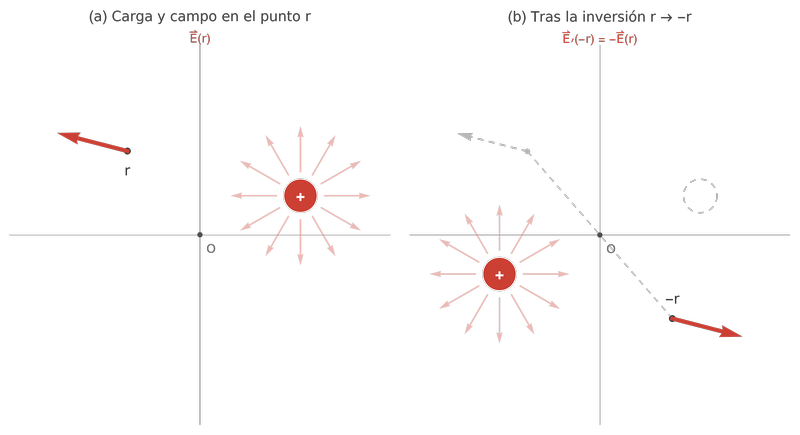
\includegraphics[width=0.95\textwidth]{imagenes/tema2/T2_4_paridad_foton_b.png}
    \caption{Una carga y su campo en un punto $\vec r$ antes de la inversión. Después de invertir, la carga pasa a $-\vec A_0$ y el campo en $-\vec r$ es el opuesto del original. Es la imagen de $\vec E(\vec r)\to-\vec E(-\vec r)$, con el punto simétrico y su traza dibujados en gris.}
    \label{fig:T2_4_paridad_foton_b}
\end{figure}

\subsubsection*{2. Comportamiento del potencial vectorial $\vec{A}(\vec{r},t)$}

En el espacio libre de fuentes y cargas, el campo eléctrico se expresa a través de los potenciales electromagnéticos como:
\begin{equation}
    \vec{E}(\vec{r},t) = -\vec{\nabla}\phi(\vec{r},t) - \frac{1}{c} \frac{\partial \vec{A}(\vec{r},t)}{\partial t}
\end{equation}

Fijando la norma en el \textbf{gauge de Coulomb} ($\vec{\nabla} \cdot \vec{A} = 0$ y $\phi = 0$), el campo eléctrico se reduce unívocamente a la derivada temporal del potencial vectorial:
\begin{equation}
    \vec{E}(\vec{r},t) = -\frac{1}{c} \frac{\partial \vec{A}(\vec{r},t)}{\partial t}
\end{equation}

Puesto que el operador de derivada temporal $\frac{\partial}{\partial t}$ no actúa sobre las coordenadas de posición y no altera las propiedades de transformación espacial, la ley de transformación de $\vec{E}(\vec{r},t)$ exige que el potencial vector $\vec{A}(\vec{r},t)$ sea también un \textbf{vector polar}:
\begin{equation}
    \vec{A}(\vec{r},t) \longrightarrow -\vec{A}(-\vec{r},t)
\end{equation}

\begin{figure}[htbp]
    \centering
    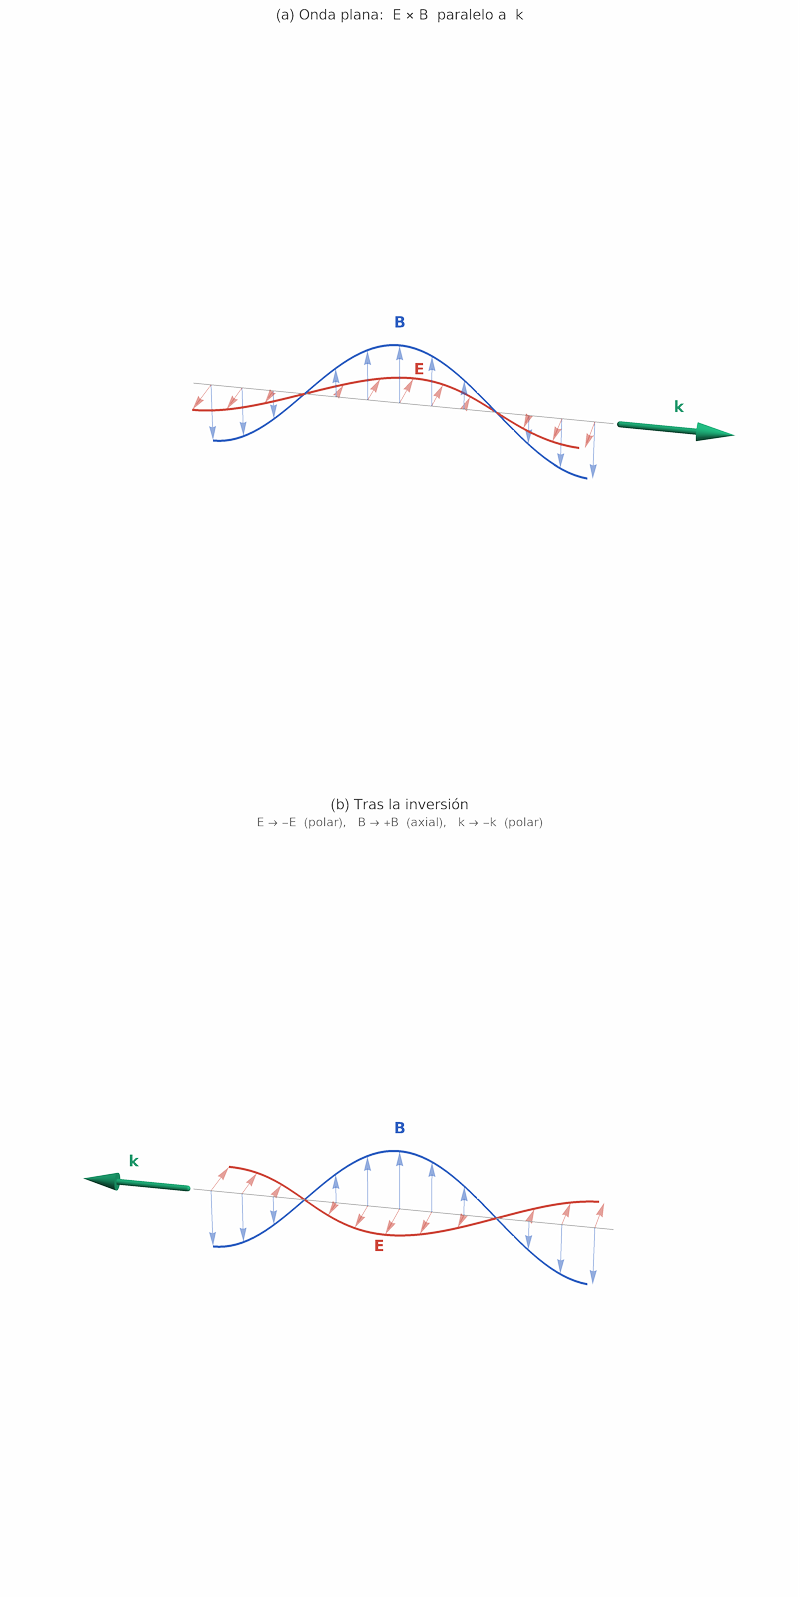
\includegraphics[width=0.95\textwidth]{imagenes/tema2/T2_4_paridad_foton_c.png}
    \caption{Una instantánea de $\vec E$, $\vec B$ y $\vec k$ antes y después de la inversión. $\vec E$ y $\vec k$ se invierten, $\vec B$ no, y aun así sigue cumpliéndose $\vec E\times\vec B\parallel\vec k$, así que la onda invertida es una solución válida.}
    \label{fig:T2_4_paridad_foton_c}
\end{figure}

\subsubsection*{3. Paridad intrínseca}

En la electrodinámica cuántica, el fotón ($\gamma$) es el cuanto de energía y momento asociado a la cuantización del campo de radiación vectorial $\vec{A}(\vec{r},t)$. 

Al heredar directamente la norma de transformación de paridad del potencial vectorial $\vec{A}(\vec{r},t)$, la paridad intrínseca del fotón viene dada por:
\begin{concepto}[Paridad del fotón]
\begin{equation}
    P_\gamma = -1
\end{equation}
\end{concepto}

\begin{figure}[htbp]
    \centering
    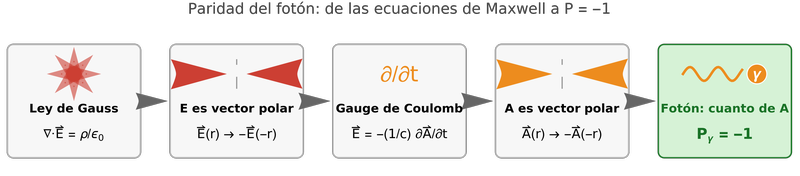
\includegraphics[width=0.95\textwidth]{imagenes/tema2/T2_4_paridad_foton_d.png}
    \caption{Cadena lógica: Gauss, $\vec E$ polar, gauge de Coulomb, $\vec A$ polar y fotón con $P_\gamma=-1$. Es el esquema de tus tres subsecciones. La última caja está en verde porque es el resultado.}
    \label{fig:T2_4_paridad_foton_d}
\end{figure}

\newpage
%=============================================================
% Sección 4. Subsección d) DETERMINACIÓN EXPERIMENTAL DE LA PARIDAD DEL PION
%=============================================================
\subsection{Determinación experimental de la paridad del pion}

La paridad del pión ($\pi$) puede deducirse teóricamente en el marco del modelo de quarks como un estado ligado quark-antiquark ($q\bar{q}$). Al ser el mesón más ligero con momento angular orbital relativo nulo ($L_{q\bar{q}} = 0$), su paridad intrínseca viene dada por el producto de las paridades del quark y del antiquark:
\begin{equation}
    P_\pi = P_q P_{\bar{q}} (-1)^{L_{q\bar{q}}} = (+1)(-1)(-1)^0 = -1
\end{equation}

Sin embargo, la paridad del pión se determinó experimentalmente con anterioridad al desarrollo del modelo de quarks (Panofsky et al., 1951) mediante el estudio de la captura piónica por deuterones en reposo:
\begin{equation}
    \pi^- + d \longrightarrow n + n
\end{equation}

\begin{figure}[htbp]
    \centering
    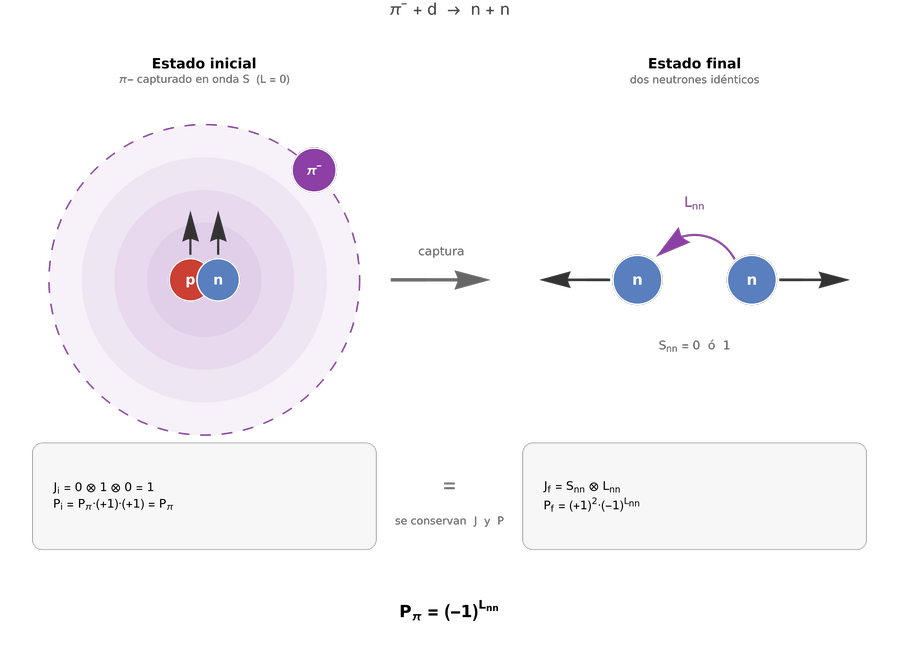
\includegraphics[width=0.95\textwidth]{imagenes/tema2/T2_4_paridad_pion_a.png}
    \caption{Experimento: A la izquierda, el pión en órbita s alrededor del deuterón, con los dos espines alineados ($J_d=1$). A la derecha, los dos neutrones que salen en direcciones opuestas, con su momento angular relativo $L_{nn}$. Los dos recuadros inferiores resumen el balance de $J$ y $P$ que lleva a $P_\pi=(-1)^{L_{nn}}$.}
    \label{fig:T2_4_paridad_pion_a}
\end{figure}

\newpage
\subsubsection*{1. Análisis de conservación de la paridad}

El deuterón ($d$) es un estado ligado protón-neutrón ($pn$) en onda $S$ ($L_{pn} = 0$) con espín total $J_d = 1$ y paridad positiva, $J_d^P = 1^+$. El protón y el neutrón son fermiones con paridad intrínseca positiva por convenio ($P_p = P_n = +1$).

Imponiendo la conservación de la paridad espacial en la reacción de captura:
\begin{equation}
    P_i = P_{\pi^-} P_d (-1)^{L_{\pi^- d}} = P_f = (P_n)^2 (-1)^{L_{nn}}
\end{equation}

Dado que $P_d = +1$ y $P_n = +1$, la ecuación se simplifica a:
\begin{equation}
    P_{\pi^-} (-1)^{L_{\pi^- d}} = (-1)^{L_{nn}}
\end{equation}

En el experimento, los piones negativos son frenados en el deuterio líquido hasta ser capturados en órbitas atómicas de baja energía (onda $S$, $L_{\pi^- d} = 0$). Por tanto, $(-1)^{L_{\pi^- d}} = (-1)^0 = +1$, lo que reduce la paridad del pión a:
\begin{equation}
    P_{\pi^-} = (-1)^{L_{nn}}
\end{equation}

\subsubsection*{2. Conservación del momento angular total y principio de Pauli}

Para determinar si $L_{nn}$ es par o impar, imponemos la conservación del momento angular total $J$ y las restricciones impuestas por la estadística de Fermi-Dirac sobre el estado final de dos neutrones idénticos.

\paragraph{Momento angular del estado inicial ($J_i$):}
\begin{equation}
    \vec{J}_i = \vec{J}_{\pi^-} \otimes \vec{J}_d \otimes \vec{L}_{\pi^- d} = 0 \otimes 1 \otimes 0 \implies J_i = 1
\end{equation}

\paragraph{Momento angular del estado final ($J_f$):}
El estado final consta de dos neutrones de espín $1/2$. El momento angular total resulta de acoplar el espín total de los dos neutrones $S_{nn}$ con su momento angular orbital relativo $L_{nn}$:
\begin{equation}
    \vec{S}_{nn} = \frac{1}{2} \otimes \frac{1}{2} = 0 \oplus 1 \implies J_f = (0 \oplus 1) \otimes L_{nn}
\end{equation}

\paragraph{Restricción de antisimetría por fermiones idénticos:}
La función de onda total de los dos neutrones $\Psi_{nn} = \Psi_{\text{espacial}} \otimes \Psi_{\text{espín}}$ debe ser estrictamente \textbf{antisimétrica} bajo el intercambio de las dos partículas:

\begin{enumerate}
    \item \textbf{Singlete de espín ($S_{nn} = 0$):}
    \begin{itemize}
        \item La parte de espín es antisimétrica ($\Psi_{\text{espín}}$ antisimétrica).
        \item Por el principio de Pauli, la parte espacial debe ser simétrica ($\Psi_{\text{espacial}}$ simétrica) $\implies L_{nn}$ debe ser \textbf{par} ($L_{nn} = 0, 2, 4, \dots$).
        \item Acoplamiento de momento angular: $J_f = S_{nn} \otimes L_{nn} = 0 \otimes L_{nn} = L_{nn}$.
        \item Para conservar el momento angular ($J_f = J_i = 1$), se requeriría $L_{nn} = 1$. Sin embargo, $L_{nn} = 1$ es impar, lo cual entra en contradicción directa con la simetría de Pauli. Por consiguiente, el canal $S_{nn} = 0$ está **estrictamente prohibido**.
    \end{itemize}

    \item \textbf{Triplete de espín ($S_{nn} = 1$):}
    \begin{itemize}
        \item La parte de espín es simétrica ($\Psi_{\text{espín}}$ simétrica).
        \item Por el principio de Pauli, la parte espacial debe ser antisimétrica ($\Psi_{\text{espacial}}$ antisimétrica) $\implies L_{nn}$ debe ser \textbf{impar} ($L_{nn} = 1, 3, 5, \dots$).
        \item Acoplamiento de momento angular: $J_f = 1 \otimes L_{nn}$. Para $L_{nn} = 1$, la suma vectorial da:
        \begin{equation}
            1 \otimes 1 = 0 \oplus 1 \oplus 2 \supset J_i = 1
        \end{equation}
        El valor $J_f = 1$ está físicamente contenido en la suma vectorial.
    \end{itemize}
\end{enumerate}

Por lo tanto, la única configuración del estado final compatible simultáneamente con la conservación del momento angular y la antisimetría del estado de dos fermiones idénticos es la correspondiente a $S_{nn} = 1$ y momento angular orbital **impar** $L_{nn} = 1$.

\newpage
\begin{figure}[htbp]
    \centering
    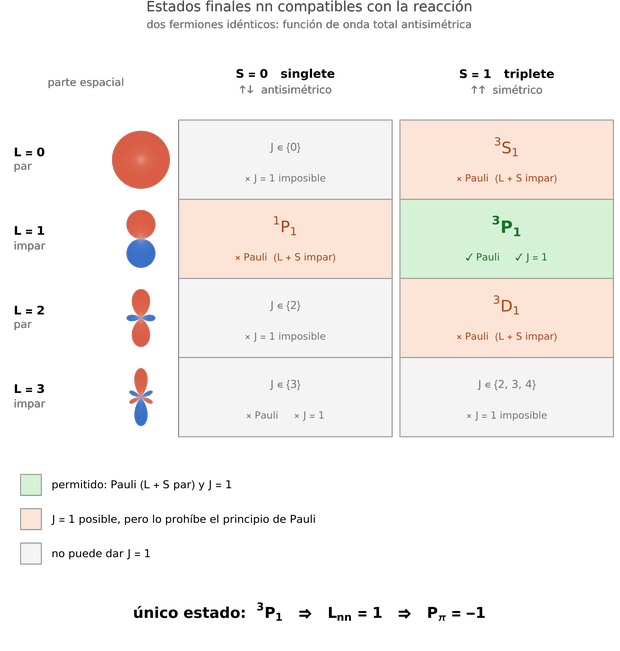
\includegraphics[width=0.75\textwidth]{imagenes/tema2/T2_4_paridad_pion_b.png}
    \caption{Tabla de los estados $(S_{nn},L_{nn})$: Las filas llevan el signo de la función espacial: lóbulos rojos y azules, simétricos si $L$ es par y antisimétricos si es impar. En verde queda solo ${}^3P_1$. En naranja quedan los estados con $J=1$ que prohíbe Pauli (${}^3S_1$, ${}^1P_1$, ${}^3D_1$), y en gris los que no pueden dar $J=1$.}
    \label{fig:T2_4_paridad_pion_b}
\end{figure}

\newpage
\subsubsection*{3. Conclusión y discusión experimental}

Sustituyendo el valor $L_{nn} = 1$ en la relación de paridad obtenida:
\begin{equation}
    P_{\pi^-} = (-1)^{L_{nn}} = (-1)^1 = -1
\end{equation}

\begin{concepto}[Paridad del pion]
La captura piónica en el deuterón demuestra experimentalmente que el pión negativo es una partícula de paridad negativa ($P = -1$), clasificándose como un mesón \textbf{pseudoescalar} ($J^P = 0^-$).
\end{concepto}

\begin{observacion}[Interpretación de la medida experimental]
El diseño experimental original planteó verificar la tasa de reacción de captura piónica a muy bajas energías ($L_{\pi^- d} = 0$). Si la paridad del pión hubiese sido positiva ($P_{\pi^-} = +1$), la reacción habría exigido un estado final con $L_{nn}$ par, lo cual habría impedido conservar el momento angular total ($J_i = 1$) bajo la restricción del principio de Pauli, prohibiendo la reacción en onda $S$.

La observación experimental de una elevada sección eficaz de captura de piones en reposo confirmó que el proceso ocurre eficientemente en onda $S$, demostrando de forma definitiva que la paridad del pión es negativa y que la paridad espacial se conserva en la interacción fuerte.
\end{observacion}

\begin{figure}[htbp]
    \centering
    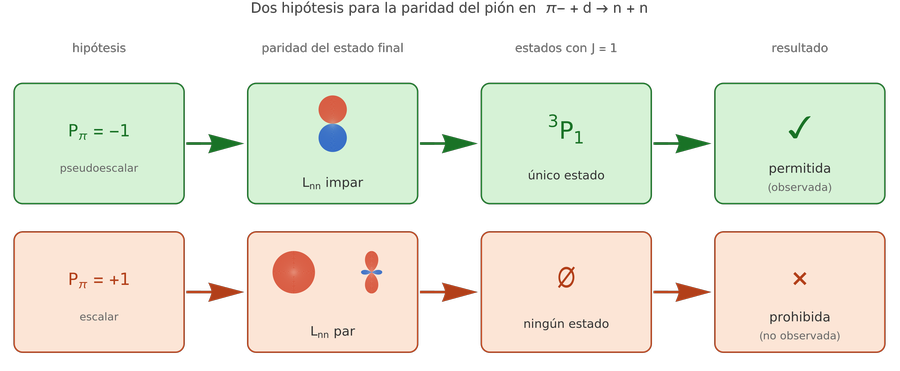
\includegraphics[width=0.95\textwidth]{imagenes/tema2/T2_4_paridad_pion_c.png}
    \caption{Compara $P_\pi=-1$ ($L_{nn}$ impar, estado ${}^3P_1$, reacción permitida y observada) con $P_\pi=+1$ ($L_{nn}$ par, ningún estado con $J=1$, reacción prohibida). Es la imagen de tu cuadro «Interpretación de la medida experimental».}
    \label{fig:T2_4_paridad_pion_c}
\end{figure}

\newpage
%=============================================================
% Sección 5. CONJUGACIÓN DE CARGA
%=============================================================
\section{Conjugación de carga}

La \textbf{conjugación de carga} es una simetría discreta representada por el operador cuántico $\hat{C}$, cuya acción transforma una partícula en su correspondiente antipartícula revirtiendo el signo de todos sus números cuánticos aditivos (carga eléctrica, número bariónico, números leptónicos, extrañeza, etc.), sin alterar sus grados de libertad espaciales (posición, momento) ni su espín intrínseco:
\begin{equation}
    \hat{C} |p, \vec{r}, \vec{s}, Q\rangle = |p, \vec{r}, \vec{s}, -Q\rangle
\end{equation}
\begin{figure}[htbp]
    \centering
    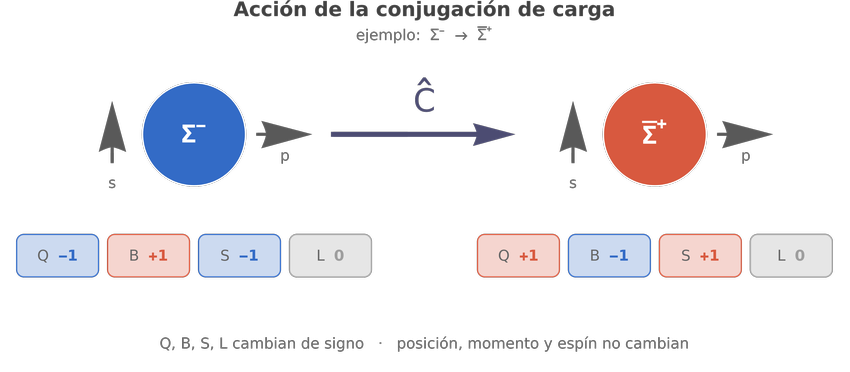
\includegraphics[width=0.65\textwidth]{imagenes/tema2/T2_5_a.png}
    \caption{Acción de $\hat{C}$.}
    \label{fig:T2_5_a}
\end{figure}

Sus propiedades algebraicas fundamentales son:
\begin{itemize}
    \item \textbf{Hermiticidad:} Al corresponder a una cantidad físicamente observable, el operador $\hat{C}$ es hermítico:
    \begin{equation}
        \hat{C}^\dagger = \hat{C}
    \end{equation}
    \item \textbf{Involución e Inversión:} Aplicar dos veces consecutivas la conjugación de carga devuelve el estado original:
    \begin{equation}
        \hat{C}^2 = \mathbb{I} \implies \hat{C}^{-1} = \hat{C}
    \end{equation}
    \item \textbf{Unitariedad:} Como $\hat{C}^{-1} = \hat{C}^\dagger$, el operador es unitario y conserva la norma de los estados cuánticos.
    \item \textbf{Autovalores:} Los autovalores $C$ de $\hat{C}$ cumplen:
    \begin{equation}
        \hat{C}^2 |\Psi\rangle = C^2 |\Psi\rangle = |\Psi\rangle \implies C^2 = 1 \implies C = \pm 1
    \end{equation}
\end{itemize}

\begin{figure}[htbp]
    \centering
    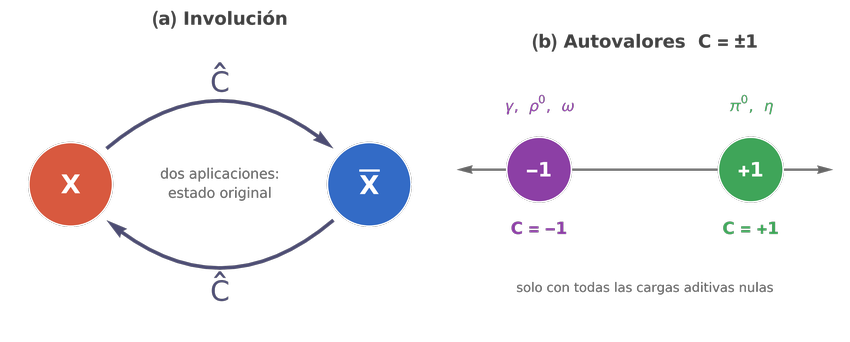
\includegraphics[width=0.75\textwidth]{imagenes/tema2/T2_5_b.png}
    \caption{Involución y autovalores $\pm1$.}
    \label{fig:T2_5_b}
\end{figure}

La conjugación de carga es una simetría exacta de las interacciones fuerte y electromagnética ($[\hat{C}, H_{\text{fuerte}}] = 0$, $[\hat{C}, H_{\text{em}}] = 0$), pero se viola explícitamente en la interacción débil.

\newpage
\subsection{Relación de anticonmutación con los operadores de carga aditiva}

Sea $|\Psi_Q\rangle$ un autoestado del operador de carga eléctrica $\hat{Q}$ con autovalor $Q$:
\begin{equation}
    \hat{Q} |\Psi_Q\rangle = Q |\Psi_Q\rangle
\end{equation}

Aplicamos secuencialmente los operadores $\hat{C}$ y $\hat{Q}$:
\begin{enumerate}
    \item Si actuamos primero con $\hat{Q}$ y posteriormente con $\hat{C}$:
    \begin{equation}
        \hat{C} (\hat{Q} |\Psi_Q\rangle) = \hat{C} (Q |\Psi_Q\rangle) = Q \hat{C} |\Psi_Q\rangle = Q |\Psi_{-Q}\rangle
    \end{equation}
    \item Si actuamos primero con $\hat{C}$ transformando la carga del estado $|\Psi_Q\rangle \to |\Psi_{-Q}\rangle$, y posteriormente medimos la carga con $\hat{Q}$:
    \begin{equation}
        \hat{Q} (\hat{C} |\Psi_Q\rangle) = \hat{Q} |\Psi_{-Q}\rangle = -Q |\Psi_{-Q}\rangle
    \end{equation}
\end{enumerate}

\begin{figure}[htbp]
    \centering
    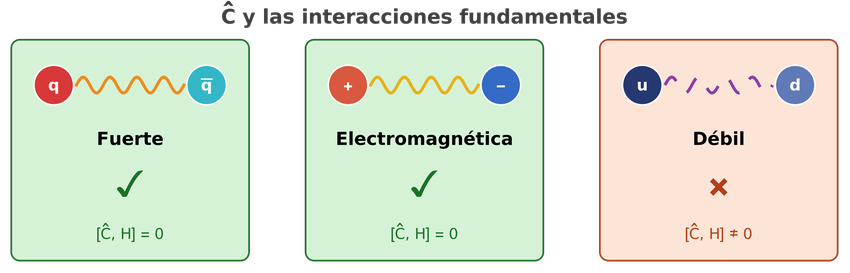
\includegraphics[width=0.7\textwidth]{imagenes/tema2/T2_5_c.png}
    \caption{$\hat{C}$ y las tres interacciones.}
    \label{fig:T2_5_c}
\end{figure}

Igualando ambas expresiones para cualquier estado arbitrario, deducimos la relación de anticonmutación fundamental:
\begin{equation}
    \hat{C} \hat{Q} = -\hat{Q} \hat{C} \iff \{\hat{C}, \hat{Q}\} = 0 \iff \hat{C} \hat{Q} \hat{C}^{-1} = -\hat{Q}
\end{equation}

De forma totalmente análoga, el operador $\hat{C}$ anticonmuta con todos los operadores asociados a cargas aditivas conservadas:
\begin{itemize}
    \item Número bariónico ($B$): $\hat{C} \hat{B} \hat{C}^{-1} = -\hat{B}$
    \item Números leptónicos ($L_i$, con $i = e, \mu, \tau$): $\hat{C} \hat{L}_i \hat{C}^{-1} = -\hat{L}_i$
    \item Extrañeza ($S$), Encanto ($\mathcal{C}$), Bottomness ($\mathcal{B}$) y Topness ($\mathcal{T}$): $\hat{C} \hat{S} \hat{C}^{-1} = -\hat{S}$, etc.
\end{itemize}

\begin{figure}[htbp]
    \centering
    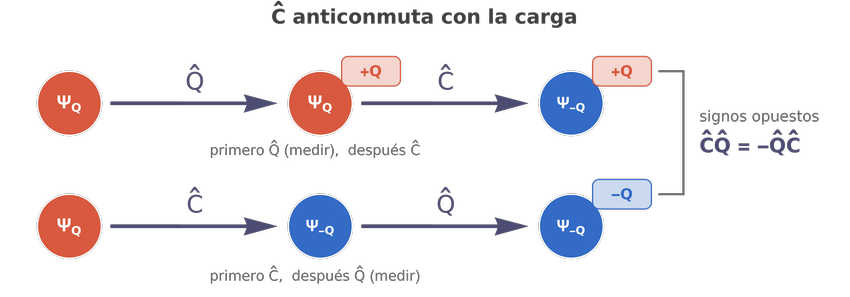
\includegraphics[width=0.7\textwidth]{imagenes/tema2/T2_5_d.png}
    \caption{Anticonmutación}
    \label{fig:T2_5_d}
\end{figure}

\newpage
\begin{concepto}[Condición de existencia de autoestados de $\hat{C}$]
Para que un estado cuántico $|\Psi\rangle$ sea autoestado del operador conjugación de carga $\hat{C}$, es \textbf{estrictamente necesario} que todos sus números cuánticos aditivos que cambian de signo bajo $\hat{C}$ sean nulos:
\begin{equation}
    Q = B = L_e = L_\mu = L_\tau = S = \mathcal{C} = \mathcal{B} = \mathcal{T} = 0
\end{equation}
Esta condición es \textbf{necesaria pero no suficiente}: la anulación de estas cargas no garantiza por sí sola que el estado sea autoestado de $\hat{C}$ (por ejemplo, el kaón neutro $K^0$ tiene $Q=B=L=0$, pero posee extrañeza $S=+1 \neq 0$, por lo que no es autoestado de $\hat{C}$).

En sistemas hadrónicos, los candidatos naturales a autoestados de $\hat{C}$ son los mesones neutros con sabor neto nulo ($\pi^0, \eta, \eta', \rho^0, \omega, \phi, J/\psi, \Upsilon$) y los fotones ($\gamma$).

Los estados con $C$ bien definido se etiquetan con los números cuánticos $J^{PC}$, donde $J$ es el espín total, $P$ la paridad espacial y $C$ la paridad de conjugación de carga. Mientras que los piones cargados tienen $J^P = 0^-$, el pión neutro posee $J^{PC} = 0^{-+}$.
\end{concepto}

\begin{figure}[htbp]
    \centering
    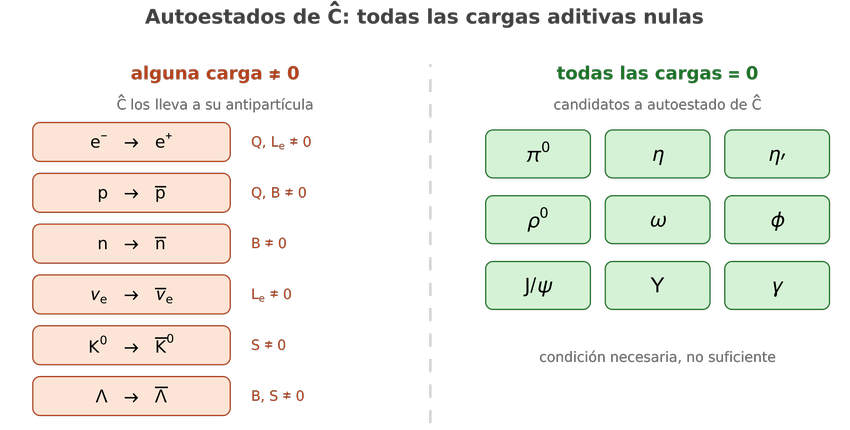
\includegraphics[width=0.85\textwidth]{imagenes/tema2/T2_5_e.png}
    \caption{Condición de autoestado.}
    \label{fig:T2_5_e}
\end{figure}

\newpage
\subsection{Conjugación de carga del pión neutro}

El pión neutro ($\pi^0$) se desintegra dominantemente mediante la interacción electromagnética en dos fotones:
\begin{equation}
    \pi^0 \longrightarrow \gamma + \gamma \quad (BR \approx 0.998)
\end{equation}

Puesto que la interacción electromagnética conserva la conjugación de carga ($[\hat{C}, H_{\text{em}}] = 0$), la paridad de conjugación de carga del estado inicial debe coincidir con la del estado final de dos fotones:
\begin{equation}
    C_{\pi^0} = C_{\gamma\gamma} = (C_\gamma)^2 = (-1)^2 = +1
\end{equation}

Por lo tanto, los números cuánticos completos del pión neutro son:
\begin{equation}
    J_{\pi^0}^{PC} = 0^{-+}
\end{equation}

\subsection{Conjugación de carga del fotón}

Clásicamente, la conjugación de carga revierte el signo de las fuentes electromagnéticas:
\begin{equation}
    \rho(\vec{r},t) \xrightarrow{\hat{C}} -\rho(\vec{r},t), \quad \vec{j}(\vec{r},t) \xrightarrow{\hat{C}} -\vec{j}(\vec{r},t)
\end{equation}

Para mantener la invariancia de forma de las ecuaciones de Maxwell de la electrodinámica:
\begin{align}
    \vec{\nabla} \cdot \vec{E}(\vec{r},t) &= \frac{1}{\varepsilon_0} \rho(\vec{r},t) \implies \vec{E}(\vec{r},t) \xrightarrow{\hat{C}} -\vec{E}(\vec{r},t) \\
    \vec{\nabla} \times \vec{B}(\vec{r},t) &= \mu_0 \vec{j}(\vec{r},t) + \mu_0 \varepsilon_0 \frac{\partial \vec{E}(\vec{r},t)}{\partial t} \implies \vec{B}(\vec{r},t) \xrightarrow{\hat{C}} -\vec{B}(\vec{r},t)
\end{align}

Expresando el campo eléctrico libre de fuentes en función del potencial vectorial $\vec{A}(\vec{r},t)$ en el gauge de Coulomb ($\phi = 0$):
\begin{equation}
    \vec{E}(\vec{r},t) = -\frac{1}{c} \frac{\partial \vec{A}(\vec{r},t)}{\partial t}
\end{equation}

La transformación impar de $\vec{E}$ bajo $\hat{C}$ exige que el potencial vectorial satisfaga:
\begin{equation}
    \vec{A}(\vec{r},t) \xrightarrow{\hat{C}} -\vec{A}(\vec{r},t)
\end{equation}

Al ser el fotón el cuanto del campo vectorial electromagnético $\vec{A}(\vec{r},t)$, hereda directamente su paridad de conjugación de carga:

\begin{figure}[htbp]
    \centering
    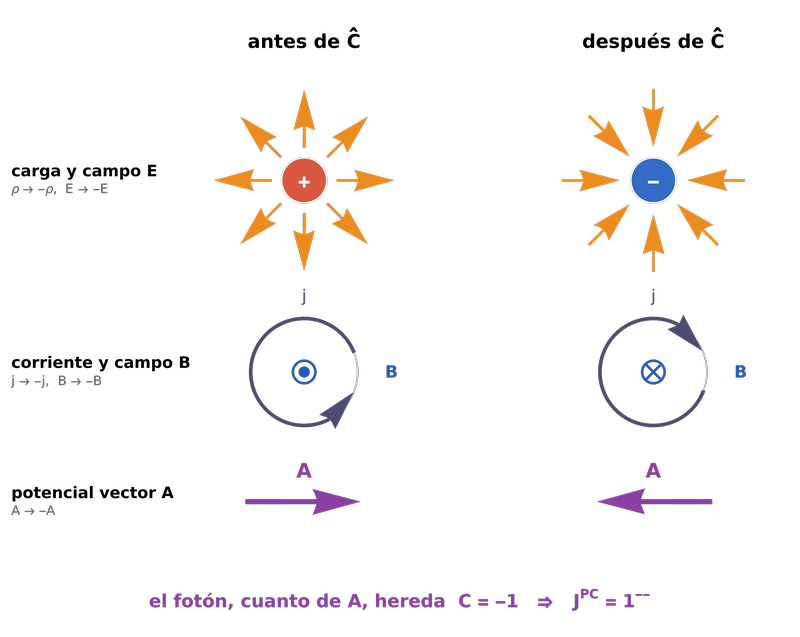
\includegraphics[width=0.45\textwidth]{imagenes/tema2/T2_5_f.png}
    \label{fig:T2_5_f}
\end{figure}

\newpage
\begin{concepto}[Conjugación de carga del fotón]
\begin{equation}
    C_\gamma = -1 \implies J_\gamma^{PC} = 1^{--}
\end{equation}
\end{concepto}

\subsubsection*{Aplicación: Prohibición de la desintegración $\pi^0 \to 3\gamma$}

\begin{figure}[htbp]
    \centering
    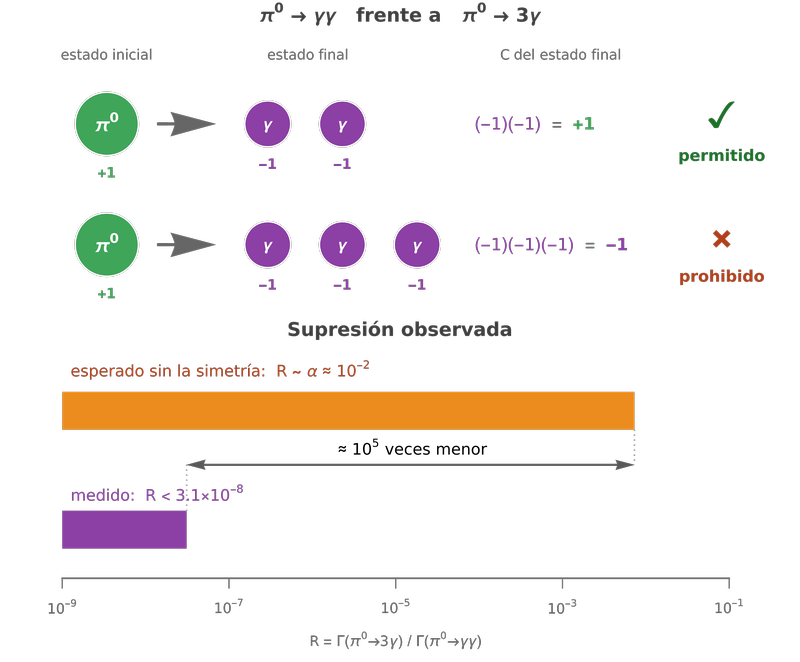
\includegraphics[width=0.75\textwidth]{imagenes/tema2/T2_5_g.png}
    \caption{$\pi^0\to\gamma+\gamma+\gamma$.}
    \label{fig:T2_5_g}
\end{figure}

La conservación de la conjugación de carga permite explicar la supresión de la desintegración del pión neutro en tres fotones:
\begin{equation}
    R = \frac{\Gamma(\pi^0 \to \gamma + \gamma + \gamma)}{\Gamma(\pi^0 \to \gamma + \gamma)}
\end{equation}

Desde el punto de vista del espacio de fases y acoplamientos electromagnéticos, un vertice adicional de fotón sugeriría teóricamente:
\begin{equation}
    R^{\text{teor}} \sim \frac{\alpha^3}{\alpha^2} = \alpha \approx 10^{-2}
\end{equation}

Sin embargo, el cota experimental es:
\begin{equation}
    R^{\text{exp}} < 3.1 \times 10^{-8}
\end{equation}

\paragraph{Explicación mediante simetría $\hat{C}$:}
\begin{itemize}
    \item Estado inicial: $C_i = C_{\pi^0} = +1$.
    \item Estado final de $n$ fotones: $C_{n\gamma} = (C_\gamma)^n = (-1)^n$.
    \begin{itemize}
        \item Para $n = 2$: $C_{2\gamma} = (-1)^2 = +1$ \quad (\checkmark \, Permitido por $\hat{C}$).
        \item Para $n = 3$: $C_{3\gamma} = (-1)^3 = -1$ \quad (\textsf{X} \, Prohibido estrictamente por conservación de $\hat{C}$).
    \end{itemize}
\end{itemize}

\newpage
\subsubsection*{Determinación del valor de $C$ para otros mesones neutros}

\begin{figure}[htbp]
    \centering
    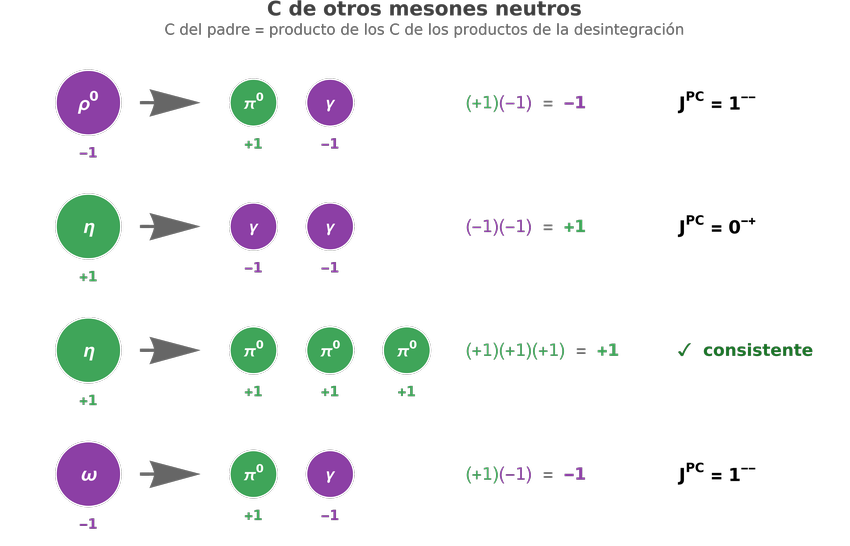
\includegraphics[width=0.85\textwidth]{imagenes/tema2/T2_5_h.png}
    \caption{Otros mesones.}
    \label{fig:T2_5_h}
\end{figure}

A partir de las propiedades conocidas de $C_{\pi^0} = +1$ y $C_\gamma = -1$, la conservación de $\hat{C}$ en desintegraciones electromagnéticas permite deducir la conjugación de carga de otros mesones neutros:

\begin{itemize}
    \item Mesón $\rho^0$: $\rho^0 \to \pi^0 + \gamma \implies C_{\rho^0} = C_{\pi^0} \cdot C_\gamma = (+1)(-1) = -1 \implies J^{PC}(\rho^0) = 1^{--}$.
    \item Mesón $\eta$: $\eta \to \gamma + \gamma \implies C_\eta = (C_\gamma)^2 = (-1)^2 = +1 \implies J^{PC}(\eta) = 0^{-+}$.
    \item Mesón $\eta$ (canal tri-piónico): $\eta \to \pi^0 + \pi^0 + \pi^0 \implies C_\eta = (C_{\pi^0})^3 = (+1)^3 = +1$ \quad (Consistente).
    \item Mesón $\omega$: $\omega \to \pi^0 + \gamma \implies C_\omega = C_{\pi^0} \cdot C_\gamma = (+1)(-1) = -1 \implies J^{PC}(\omega) = 1^{--}$.
\end{itemize}

\newpage
\subsection{Conjugación de carga del sistema partícula-antipartícula}

La conjugación de carga $\hat{C}$ tendría una utilidad física limitada si sus únicos autoestados fuesen los mesones neutros con sabor nulo y el fotón. Sin embargo, un sistema formado por una partícula y su propia antipartícula ($f\bar{f}$ o $b\bar{b}$) posee un valor nulo para todas las cargas aditivas conservadas ($Q = 0, B = 0, L = 0, S = 0$), lo que le permite constituir un autoestado del operador $\hat{C}$.

A continuación, deducimos de manera rigurosa el autovalor de conjugación de carga $C$ para un sistema partícula-antipartícula general, distinguiendo entre constituyentes fermiónicos y bosónicos.

\subsubsection{Sistemas fermiónicos ($f\bar{f}$)}

Consideremos un sistema formado por un fermión $f$ (partícula 1) y su antifermión $\bar{f}$ (partícula 2), cada uno con espín intrínseco semientero $s_f$. Para construir un autoestado de $\hat{C}$ con simetría adecuada bajo el intercambio de etiquetas, escribimos la función de onda total antisimétrica $\Psi(1,2)$ factorizada en sus partes de sabor/carga, espacial y de espín:
\begin{equation}
    \Psi(1,2) = \Psi_f(1)\Psi_{\bar{f}}(2) \, \Phi_L(\vec{r}_{12}) \, \chi_S(\xi_1,\xi_2) - \Psi_f(2)\Psi_{\bar{f}}(1) \, \Phi_L(\vec{r}_{21}) \, \chi_S(\xi_2,\xi_1)
\end{equation}
donde $\vec{r}_{12} = \vec{r}_1 - \vec{r}_2$ es la coordenada relativa, $L$ es el momento angular orbital relativo y $S$ es el espín total del sistema acoplado.

El operador de conjugación de carga $\hat{C}$ intercambia el estado de partícula por el de antipartícula:
\begin{equation}
    \hat{C} \left[ \Psi_f(1) \Psi_{\bar{f}}(2) \right] = \Psi_{\bar{f}}(1) \Psi_f(2) = \Psi_f(2) \Psi_{\bar{f}}(1)
\end{equation}

Aplicando $\hat{C}$ a la función de onda total $\Psi(1,2)$:
\begin{align}
    \hat{C}\Psi(1,2) &= \Psi_{\bar{f}}(1)\Psi_f(2) \, \Phi_L(\vec{r}_{12}) \, \chi_S(\xi_1,\xi_2) - \Psi_{\bar{f}}(2)\Psi_f(1) \, \Phi_L(\vec{r}_{21}) \, \chi_S(\xi_2,\xi_1) \nonumber \\
    &= \Psi_f(2)\Psi_{\bar{f}}(1) \, \Phi_L(\vec{r}_{12}) \, \chi_S(\xi_1,\xi_2) - \Psi_f(1)\Psi_{\bar{f}}(2) \, \Phi_L(\vec{r}_{21}) \, \chi_S(\xi_2,\xi_1) \nonumber \\
    &= -\Psi_f(1)\Psi_{\bar{f}}(2) \, \Phi_L(\vec{r}_{21}) \, \chi_S(\xi_2,\xi_1) + \Psi_f(2)\Psi_{\bar{f}}(1) \, \Phi_L(\vec{r}_{12}) \, \chi_S(\xi_1,\xi_2)
\end{align}

Utilizamos las propiedades de simetría bajo intercambio de las funciones espacial y de espín:
\begin{enumerate}
    \item \textbf{Inversión espacial:} $\Phi_L(\vec{r}_{21}) = (-1)^L \Phi_L(\vec{r}_{12})$.
    \item \textbf{Intercambio de espín:} Para dos partículas de espín $s_f$ acopladas a espín total $S$, la simetría de intercambio de los estados de espín satisface:
    \begin{equation}
        \chi_S(\xi_2,\xi_1) = (-1)^{S - 2s_f} \chi_S(\xi_1,\xi_2)
    \end{equation}
\end{enumerate}

Sustituyendo ambas relaciones de intercambio en la acción de $\hat{C}$:
\begin{align}
    \hat{C}\Psi(1,2) &= -(-1)^L (-1)^{S - 2s_f} \left[ \Psi_f(1)\Psi_{\bar{f}}(2) \, \Phi_L(\vec{r}_{12}) \, \chi_S(\xi_1,\xi_2) - \Psi_f(2)\Psi_{\bar{f}}(1) \, \Phi_L(\vec{r}_{21}) \, \chi_S(\xi_2,\xi_1) \right] \nonumber \\
    &= -(-1)^L (-1)^{S - 2s_f} \Psi(1,2)
\end{align}

\newpage
\subsection{2.c.- Conjugación de carga del sistema partícula-antipartícula}

La conjugación de carga sería una simetría de aplicabilidad restringida si sus autoestados se limitasen únicamente a los fotones y a los mesones neutros sin sabores pesados. Sin embargo, un sistema compuesto por una partícula y su propia antipartícula (como un par $f\bar{f}$ de fermiones o $b\bar{b}$ de bosones) posee valores opuestos para todos sus números cuánticos aditivos (carga eléctrica $Q$, número bariónico $B$, números leptónicos $L_i$, extrañeza $S$, etc.), de modo que sus cargas netas se anulan idénticamente:
\begin{equation}
    Q_{\text{total}} = B_{\text{total}} = L_i = S = 0
\end{equation}

Por consiguiente, un sistema partícula-antipartícula constituye un candidato natural para ser autoestado del operador conjugación de carga $\hat{C}$. A continuación, construimos de manera explícita los autovalores de $\hat{C}$ para sistemas fermiónicos y bosónicos.

\subsubsection*{1. Sistemas fermiónicos ($f\bar{f}$)}

Consideremos un sistema compuesto por un fermión $f$ y su antifermión $\bar{f}$, ambos de espín $s_f$ (con $s_f$ semientero). Para construir un estado cuántico físico $\Psi(1,2)$ con propiedades de simetría bien definidas bajo intercambio y conjugación, combinamos las partes espacial, de espín y de carga.

La función de onda total antisimetrizada bajo el intercambio de las partículas $1$ y $2$ se escribe como:
\begin{equation}
    \Psi(1,2) = \frac{1}{\sqrt{2}} \left[ \Psi_f(1) \Psi_{\bar{f}}(2) \Phi_L(\vec{r}_{12}) \chi_S(\xi_1, \xi_2) - \Psi_f(2) \Psi_{\bar{f}}(1) \Phi_L(\vec{r}_{21}) \chi_S(\xi_2, \xi_1) \right]
\end{equation}
donde $\Phi_L(\vec{r}_{12})$ representa la función de onda espacial relativa de momento angular orbital $L$, $\chi_S(\xi_1, \xi_2)$ la función del espín acoplado total $S$, y los estados de carga satisfacen la acción del operador conjugación:
\begin{equation}
    \hat{C} \left[ \Psi_f(1) \Psi_{\bar{f}}(2) \right] = \Psi_{\bar{f}}(1) \Psi_f(2)
\end{equation}

Aplicando el operador $\hat{C}$ sobre la función de onda total $\Psi(1,2)$:
\begin{align}
    \hat{C} \Psi(1,2) &= \frac{1}{\sqrt{2}} \left[ \Psi_{\bar{f}}(1) \Psi_f(2) \Phi_L(\vec{r}_{12}) \chi_S(\xi_1, \xi_2) - \Psi_{\bar{f}}(2) \Psi_f(1) \Phi_L(\vec{r}_{21}) \chi_S(\xi_2, \xi_1) \right] \nonumber \\
    &= \frac{1}{\sqrt{2}} \left[ -\Psi_f(1) \Psi_{\bar{f}}(2) \Phi_L(\vec{r}_{21}) \chi_S(\xi_2, \xi_1) + \Psi_f(2) \Psi_{\bar{f}}(1) \Phi_L(\vec{r}_{12}) \chi_S(\xi_1, \xi_2) \right]
\end{align}

Utilizando las propiedades de simetría de la parte espacial y de espín bajo permuta de coordenadas:
\begin{align}
    \Phi_L(\vec{r}_{21}) &= (-1)^L \Phi_L(\vec{r}_{12}) \\
    \chi_S(\xi_2, \xi_1) &= (-1)^{S - 2s_f} \chi_S(\xi_1, \xi_2)
\end{align}

Sustituyendo estas relaciones en la transformación de paridad de carga:
\begin{align}
    \hat{C} \Psi(1,2) &= \frac{1}{\sqrt{2}} \left[ -(-1)^L (-1)^{S-2s_f} \Psi_f(1) \Psi_{\bar{f}}(2) \Phi_L(\vec{r}_{12}) \chi_S(\xi_1, \xi_2) \right. \nonumber \\
    &\quad \left. + (-1)^L (-1)^{S-2s_f} \Psi_f(2) \Psi_{\bar{f}}(1) \Phi_L(\vec{r}_{21}) \chi_S(\xi_2, \xi_1) \right] \nonumber \\
    &= -(-1)^L (-1)^{S - 2s_f} \Psi(1,2)
\end{align}

Dado que para fermiones el espín $s_f$ es semientero ($s_f = 1/2, 3/2, \dots$), $2s_f$ es estrictamente un número entero impar ($2s_f \in \mathbb{Z}_{\text{impar}}$). Por ende:
\begin{equation}
    (-1)^{-2s_f} = -1 \implies -(-1)^{-2s_f} = -(-1) = +1
\end{equation}

Sustituyendo este factor de signo en la ecuación de autovalores, obtenemos:
\begin{equation}
    \hat{C} \Psi(1,2) = (-1)^{L+S} \Psi(1,2)
\end{equation}

\subsubsection*{2. Sistemas bosónicos ($b\bar{b}$)}

Para un sistema constituido por un bosón y su antibosón ($b\bar{b}$), ambos de espín entero $s_b$, la función de onda total $\Psi(1,2)$ debe ser simétrica bajo el intercambio completo de las dos partículas. La función de onda simetrizada es:
\begin{equation}
    \Psi(1,2) = \frac{1}{\sqrt{2}} \left[ \Psi_b(1) \Psi_{\bar{b}}(2) \Phi_L(\vec{r}_{12}) \chi_S(\xi_1, \xi_2) + \Psi_b(2) \Psi_{\bar{b}}(1) \Phi_L(\vec{r}_{21}) \chi_S(\xi_2, \xi_1) \right]
\end{equation}

Aplicando el operador de conjugación de carga $\hat{C}$ e introduciendo la simetría espacial $(-1)^L$ y de espín $(-1)^{S - 2s_b}$:
\begin{equation}
    \hat{C} \Psi(1,2) = (-1)^L (-1)^{S - 2s_b} \Psi(1,2)
\end{equation}

Dado que para bosones el espín $s_b$ es entero ($s_b = 0, 1, 2, \dots$), la cantidad $2s_b$ es un número entero par ($2s_b \in \mathbb{Z}_{\text{par}}$), lo que implica $(-1)^{-2s_b} = +1$. Por lo tanto:
\begin{equation}
    \hat{C} \Psi(1,2) = (-1)^{L+S} \Psi(1,2)
\end{equation}

\begin{concepto}[Fórmula universal de conjugación de carga para $f\bar{f}$ y $b\bar{b}$]
Independientemente del carácter fermiónico o bosónico de las partículas constituyentes, el autovalor de la conjugación de carga para cualquier sistema neutro partícula-antipartícula en un estado de momento angular orbital $L$ y espín total $S$ viene dado por:
\begin{equation}
    C = (-1)^{L+S}
\end{equation}
\end{concepto}

\subsubsection*{3. Verificación experimental en el Positronio ($e^+ e^-$)}

El \textbf{positronio} es un estado ligado electromagnético formado por un electrón y un positrón ($e^+ e^-$), con momento angular orbital relativo fundamental $L = 0$ (onda $S$). Su estudio experimental constituye una prueba directa de la conservación de la conjugación de carga en la interacción electromagnética.

El positronio presenta dos estados fundamentales según su configuración de espín total:

\paragraph{1. Parapositronio ($^1S_0$):}
Estado singlete de espín ($S = 0, L = 0$). Su autovalor de conjugación de carga es:
\begin{equation}
    C_{[e^+ e^-(^1S_0)]} = (-1)^{0+0} = +1
\end{equation}

Analizamos sus canales de desintegración electromagnética en fotones:
\begin{itemize}
    \item \textbf{Canal de 2 fotones ($2\gamma$):} $C_{2\gamma} = (C_\gamma)^2 = (-1)^2 = +1$ \quad (\checkmark \, Permitido por $\hat{C}$).
    \item \textbf{Canal de 3 fotones ($3\gamma$):} $C_{3\gamma} = (C_\gamma)^3 = (-1)^3 = -1$ \quad (\textsf{X} \, Prohibido por conservación de $\hat{C}$).
\end{itemize}

Si solo considerásemos los factores de espacio de fases y acoplamiento electromagnético, se estimaría una razón perturbativa:
\begin{equation}
    R^{\text{teor}} = \frac{\Gamma[e^+ e^-(^1S_0) \to 3\gamma]}{\Gamma[e^+ e^-(^1S_0) \to 2\gamma]} \approx \frac{\alpha^3}{\alpha^2} = \alpha \sim 10^{-2}
\end{equation}
Sin embargo, las mediciones experimentales arrojan una cota estricta:
\begin{equation}
    R^{\text{exp}} < 1 \times 10^{-5}
\end{equation}
vatios de órdenes de magnitud por debajo de la predicción ilícita. Este resultado confirma que el modo $3\gamma$ está prohibido por la simetría de conjugación de carga.

\paragraph{2. Ortopositronio ($^3S_1$):}
Estado triplete de espín ($S = 1, L = 0$). Su autovalor de conjugación de carga vale:
\begin{equation}
    C_{[e^+ e^-(^3S_1)]} = (-1)^{0+1} = -1
\end{equation}

Analizamos sus modos de desintegración:
\begin{itemize}
    \item \textbf{Canal de 2 fotones ($2\gamma$):} $C_{2\gamma} = +1 \neq -1$ \quad (\textsf{X} \, Prohibido por conservación de $\hat{C}$).
    \item \textbf{Canal de 3 fotones ($3\gamma$):} $C_{3\gamma} = -1$ \quad (\checkmark \, Permitido por $\hat{C}$).
\end{itemize}

Por consiguiente, el ortopositronio no puede desintegrarse en dos fotones y su modo principal de decaimiento electromagnético ocurre a través de la emisión de tres fotones ($^3S_1 \to 3\gamma$).

\newpage
%=====================================================
% SECCIÓN: ISOSPÍN
%=====================================================
\section{Isospín}

En la física nuclear y de partículas se observa experimentalmente que la fuerza nuclear fuerte actúa con prácticamente la misma intensidad entre dos protones ($p-p$), dos neutrones ($n-n$) o un protón y un neutrón ($p-n$), a igualdad de estado de momento angular y espín. Esta propiedad se conoce como la \textbf{independencia de carga} de la interacción fuerte.

\subsection{Motivación fenomenológica}

La evidencia empírica de esta independencia de carga se manifiesta de forma clara en dos fenómenos nucleares:

\subsubsection*{1. Núcleos espejo}
Se denominan \textbf{núcleos espejo} a aquellos pares de isóbaros que se obtienen intercambiando mutuamente el número de protones $Z$ y el número de neutrones $N$, es decir, $(Z, N) \iff (N, Z)$. Un ejemplo característico lo constituyen el litio-7 y el berilio-7:
\begin{equation}
    ^{7}_{3}\text{Li}: (Z, N) = (3, 4) \iff (Z, N) = (4, 3) : ^{7}_{4}\text{Be}
\end{equation}

Al comparar los espectros de energía de ambos núcleos, se observa una estructura de niveles prácticamente idéntica en espín, paridad y energías de excitación, salvo por una pequeña diferencia en la energía del estado fundamental asignable a la energía de repulsión culombiana entre protones.

\subsubsection*{2. Cadenas de multipletes isobáricos}
La similitud de niveles también se manifiesta en secuencias isobáricas ($A = \text{constante}$) donde se van reemplazando gradualmente protones por neutrones. Consideremos el multiplete isobárico con $A = 6$:
\begin{align}
    ^{6}_{2}\text{He} &\implies (Z, N) = (2, 4) \equiv (2, 2) + (0, 2) \quad \text{(core de } \alpha + 2n) \\
    ^{6}_{3}\text{Li} &\implies (Z, N) = (3, 3) \equiv (2, 2) + (1, 1) \quad \text{(core de } \alpha + pn) \\
    ^{6}_{4}\text{Be} &\implies (Z, N) = (4, 2) \equiv (2, 2) + (2, 0) \quad \text{(core de } \alpha + 2p)
\end{align}
Los estados fundamentales de $^{6}\text{He}$ y $^{6}\text{Be}$, junto con el primer estado excitado $0^+$ del $^{6}\text{Li}$, presentan propiedades nucleares estructuralmente análogas.

\subsection{Propiedades del protón y del neutrón}

Las propiedades estáticas fundamentales del protón y del neutrón se resumen en la siguiente tabla:

\begin{table}[htbp]
    \centering
    \begin{tabular}{lcc}
        \toprule
        \textbf{Propiedad} & \textbf{Protón ($p$)} & \textbf{Neutrón ($n$)} \\
        \midrule
        Espín y paridad ($J^P$) & $1/2^+$ & $1/2^+$ \\
        Masa en reposo ($m c^2$) & $938.272\text{ MeV}$ & $939.565\text{ MeV}$ \\
        Vida media ($\tau$) & $> 0.96 \times 10^{30}\text{ años}$ & $878.4\text{ s}$ \\
        Carga eléctrica ($Q$) & $+1\,e$ & $0$ \\
        \bottomrule
    \end{tabular}
    \caption{Propiedades fundamentales de los nucleones $p$ y $n$.}
    \label{tab:propiedades_nucleones}
\end{table}

La diferencia relativa de masa entre el protón y el neutrón es extremadamente pequeña:
\begin{equation}
    \frac{m_n - m_p}{m_p} \approx \frac{1.293\text{ MeV}}{938.272\text{ MeV}} \approx 0.14\%
\end{equation}

Esta ligera diferencia de masa, así como la inestabilidad del neutrón libre vía desintegración $\beta$ y sus distintas cargas eléctricas, se deben exclusivamente a los efectos de las \textbf{interacciones electromagnética y débil}.

\subsection{Hipótesis de Heisenberg y la analogía del espín}

En 1932, W. Heisenberg propuso que el protón y el neutrón no debían considerarse como dos partículas independientes, sino como \textbf{dos estados de carga de una misma entidad cuántica llamada nucleón} ($N$).

En ausencia de interacciones electromagnéticas y débiles, el protón y el neutrón son completamente degenerados e indistinguibles para la interacción fuerte. Esta situación es conceptualmente idéntica a la degeneración de un electrón de espín $1/2$ en ausencia de un campo magnético externo:

\begin{itemize}
    \item \textbf{Espín del electrón en mecánica cuántica:} Los dos estados proyectados de espín $|e\uparrow\rangle$ ($m_s = +1/2$) y $|e\downarrow\rangle$ ($m_s = -1/2$) forman un doblete degenerado bajo la simetría de rotación $SU(2)$. La degeneración solo se rompe al aplicar un campo magnético externo $\vec{B} \neq 0$ (efecto Zeeman).
    \item \textbf{Isospín del nucleón:} Los estados $|p\rangle$ y $|n\rangle$ forman un doblete de un nuevo espacio interno de simetría $SU(2)_I$ denominado \textbf{isospín} (o espín isotópico). La interacción electromagnética actúa como un "campo externo" que rompe la simetría $SU(2)_I$ y separa los niveles de energía del protón y del neutrón.
\end{itemize}

\begin{equation}
    \text{Nucleón }(N): \begin{cases} |p\rangle \\ |n\rangle \end{cases} \quad \xleftrightarrow{\text{Interacción EM}} \quad (\vec{B} \neq 0) \begin{cases} |e\uparrow\rangle \\ |e\downarrow\rangle \end{cases} :\text{Electrón }(e)
\end{equation}

\subsection{Formalismo matemático del Isospín}

Asociamos al nucleón un vector de operador de isospín $\hat{\vec{I}} = (\hat{I}_1, \hat{I}_2, \hat{I}_3)$ que satisface las relaciones de conmutación del álgebra de Lie $\mathfrak{su}(2)$:
\begin{equation}
    [\hat{I}_i, \hat{I}_j] = i \varepsilon_{ijk} \hat{I}_k
\end{equation}

Los operadores de isospín se representan analógicamente mediante las matrices de Pauli $\vec{\tau}$:
\begin{equation}
    \hat{\vec{I}} = \frac{1}{2} \vec{\tau}
\end{equation}

El nucleón es una partícula con número cuántico de isospín total $I = 1/2$. Sus dos estados proyectados sobre el tercer eje de isospín $I_3$ vienen dados por:
\begin{align}
    \text{Protón } |p\rangle &\equiv \left| I = \frac{1}{2}, I_3 = +\frac{1}{2} \right\rangle = \begin{pmatrix} 1 \\ 0 \end{pmatrix} \\
    \text{Neutrón } |n\rangle &\equiv \left| I = \frac{1}{2}, I_3 = -\frac{1}{2} \right\rangle = \begin{pmatrix} 0 \\ 1 \end{pmatrix}
\end{align}

La carga eléctrica operador $\hat{Q}$ para el nucleón se relaciona linealmente con la tercera componente de isospín $\hat{I}_3$ y el número bariónico $\hat{B}$ mediante la relación de Gell-Mann--Nishijima (para el sector no extraño, $S = 0$):
\begin{equation}
    \hat{Q} = \hat{I}_3 + \frac{\hat{B}}{2}
\end{equation}

Evaluando la carga para cada componente del doblete nucleónico ($B = 1$):
\begin{align}
    Q(p) &= +\frac{1}{2} + \frac{1}{2} = +1 \\
    Q(n) &= -\frac{1}{2} + \frac{1}{2} = 0
\end{align}

De este modo, la simetría de isospín proporciona un marco unificado para clasificar los hadrones en multipletes de masa ($2I + 1$ estados degenerados bajo la fuerza fuerte) y analizar las reacciones nucleares y subatómicas mediante las técnicas estándar del acoplamiento de momentos angulares (coeficientes de Clebsch-Gordan).

%=========================================================
\subsection{Analogía con el espín del electrón y formalización del Isospín}

La degeneración de estados observada en la naturaleza en ausencia de interacciones que rompan una simetría interna se explica en Mecánica Cuántica mediante la dimensión de las representaciones irreducibles del grupo $SU(2)$.

Para un sistema con momento angular $J$, el número de estados degenerados es $2J + 1$. En el caso del electrón en ausencia de campo magnético ($\vec{B} = 0$), existen dos estados de proyección de espín degenerados ($2J + 1 = 2 \implies J = 1/2$). Denotando $J \equiv S$:
\begin{align}
    |S, S_3\rangle &= \left| \frac{1}{2}, +\frac{1}{2} \right\rangle \equiv |e\uparrow\rangle \\
    |S, S_3\rangle &= \left| \frac{1}{2}, -\frac{1}{2} \right\rangle \equiv |e\downarrow\rangle
\end{align}

La indistinguibilidad entre los estados $|e\uparrow\rangle$ y $|e\downarrow\rangle$ por la interacción electromagnética pura ($\vec{B} = 0$) implica que el Hamiltoniano conmuta con el operador de espín total:
\begin{equation}
    [\hat{H}_{\text{EM}}(\vec{B}=0), \hat{\vec{S}}] = 0, \quad \text{donde } \hat{\vec{S}} = \frac{\hbar}{2} \hat{\vec{\sigma}}
\end{equation}
siendo $\hat{\vec{\sigma}}$ las matrices de Pauli. En consecuencia, el valor esperado de la energía es independiente de la proyección $S_3$:
\begin{equation}
    \langle S, S_3 | \hat{H}_{\text{EM}}(\vec{B}=0) | S, S_3 \rangle \neq f(S_3)
\end{equation}

De forma conceptualmente análoga, la invariancia de la interacción fuerte bajo el intercambio entre protones y neutrones sugiere la existencia de un nuevo grado de libertad interno descrito por una simetría de calibre global $SU(2)_I$, cuyo álgebra es isomórfica a la del espín. Este nuevo momento angular interno, denominado **isospín** ($I$), genera la degeneración del doblete nucleónico ($2I + 1 = 2 \implies I = 1/2$):
\begin{align}
    |I, I_3\rangle &= \left| \frac{1}{2}, +\frac{1}{2} \right\rangle \equiv |p\rangle \\
    |I, I_3\rangle &= \left| \frac{1}{2}, -\frac{1}{2} \right\rangle \equiv |n\rangle
\end{align}

La indistinguibilidad entre el protón y el neutrón ante la fuerza nuclear fuerte exige la conmutación entre el Hamiltoniano fuerte $\hat{H}_S$ y el vector de operadores de isospín $\hat{\vec{I}}$:
\begin{equation}
    [\hat{H}_S, \hat{\vec{I}}] = 0, \quad \text{donde } \hat{\vec{I}} = \frac{\hbar}{2} \hat{\vec{\tau}}
\end{equation}
representando $\hat{\vec{\tau}} = (\hat{\tau}_1, \hat{\tau}_2, \hat{\tau}_3)$ las matrices de Pauli en el espacio abstracto de isospín.

La tercera componente de isospín $I_3$ se relaciona directamente con la carga eléctrica $Q$ (en unidades de la carga elemental $|e|$):
\begin{equation}
    Q = I_3 + \frac{1}{2}
\end{equation}

\subsection{Álgebra de los operadores de isospín}

Los operadores de isospín son observables hermíticos ($\hat{I}_i = \hat{I}_i^\dagger$, con $i=1,2,3$) que satisfacen las relaciones de conmutación del álgebra de Lie $\mathfrak{su}(2)$:
\begin{equation}
    [\hat{I}_i, \hat{I}_j] = i \hbar \varepsilon_{ijk} \hat{I}_k
\end{equation}

El operador correspondiente al cuadrado del isospín total se define como:
\begin{equation}
    \hat{I}^2 = \sum_{i=1}^3 \hat{I}_i^2 \implies [\hat{I}^2, \hat{I}_i] = 0 \quad \forall i \in \{1, 2, 3\}
\end{equation}

Debido a estas relaciones de conmutación, es posible diagonalizar simultáneamente el operador escalón $\hat{I}^2$ y la tercera componente $\hat{I}_3$:
\begin{align}
    \hat{I}^2 |I, I_3\rangle &= \hbar^2 I(I+1) |I, I_3\rangle \\
    \hat{I}_3 |I, I_3\rangle &= \hbar I_3 |I, I_3\rangle
\end{align}

Asimismo, se definen los operadores de escalera (subida y bajada) en el espacio de isospín:
\begin{equation}
    \hat{I}_\pm = \hat{I}_x \pm i \hat{I}_y
\end{equation}
cuya acción sobre un autoestado $|I, I_3\rangle$ viene dada por:
\begin{equation}
    \hat{I}_\pm |I, I_3\rangle = \hbar \sqrt{I(I+1) - I_3(I_3 \pm 1)} \, |I, I_3 \pm 1\rangle
\end{equation}

\subsection{Demostración de la estructura de los elementos de matriz del Hamiltoniano fuerte}

A continuación se demuestra rigurosamente que la invarianza de isospín del Hamiltoniano de la interacción fuerte ($[\hat{H}_S, \hat{\vec{I}}] = 0$) simplifica la evaluación de sus elementos de matriz, reduciéndolos a la forma:
\begin{equation}
    \langle I', I_3' | \hat{H}_S | I, I_3 \rangle = A_I \, \delta_{I'I} \, \delta_{I_3'I_3}
\end{equation}

\subsubsection*{1. Proporcionalidad a $\delta_{I_3'I_3}$}

Puesto que la tercera componente de isospín conmuta con el Hamiltoniano fuerte ($[\hat{H}_S, \hat{I}_3] = 0$):
\begin{equation}
    \langle I, I_3' | [\hat{H}_S, \hat{I}_3] | I, I_3 \rangle = \langle I, I_3' | (\hat{H}_S \hat{I}_3 - \hat{I}_3 \hat{H}_S) | I, I_3 \rangle = 0
\end{equation}

Haciendo actuar $\hat{I}_3$ sobre los bra y ket correspondientes:
\begin{equation}
    \hbar (I_3 - I_3') \langle I, I_3' | \hat{H}_S | I, I_3 \rangle = 0
\end{equation}
Para cualquier par de estados con $I_3' \neq I_3$, la diferencia $(I_3 - I_3') \neq 0$, por lo que el elemento de matriz debe anularse obligatoriamente. Se concluye que:
\begin{equation}
    \langle I, I_3' | \hat{H}_S | I, I_3 \rangle \propto \delta_{I_3'I_3}
\end{equation}

\subsubsection*{2. Proporcionalidad a $\delta_{I'I}$}

Dado que el cuadrado del isospín total conmuta con el Hamiltoniano fuerte ($[\hat{H}_S, \hat{I}^2] = 0$):
\begin{equation}
    \langle I', I_3 | [\hat{H}_S, \hat{I}^2] | I, I_3 \rangle = \langle I', I_3 | (\hat{H}_S \hat{I}^2 - \hat{I}^2 \hat{H}_S) | I, I_3 \rangle = 0
\end{equation}

Evaluando los autovalores de $\hat{I}^2$:
\begin{equation}
    \hbar^2 [I(I+1) - I'(I'+1)] \langle I', I_3 | \hat{H}_S | I, I_3 \rangle = 0
\end{equation}

Factorizando el término entre corchetes:
\begin{equation}
    \hbar^2 (I - I')(I + I' + 1) \langle I', I_3 | \hat{H}_S | I, I_3 \rangle = 0
\end{equation}
Dado que $I, I' \ge 0$, el factor $(I + I' + 1)$ es estrictamente positivo y nunca se anula. Por ende, la única posibilidad de obtener un elemento de matriz no nulo es cuando $I = I'$, lo que demuestra que:
\begin{equation}
    \langle I', I_3 | \hat{H}_S | I, I_3 \rangle \propto \delta_{I'I}
\end{equation}

\subsubsection*{3. Independencia de $I_3$ ($A_I \equiv f(I)$)}

Puesto que los operadores de subida y bajada conmutan con el Hamiltoniano fuerte ($[\hat{H}_S, \hat{I}_\pm] = 0$):
\begin{equation}
    \langle I, I_3 + 1 | [\hat{H}_S, \hat{I}_+] | I, I_3 \rangle = \langle I, I_3 + 1 | (\hat{H}_S \hat{I}_+ - \hat{I}_+ \hat{H}_S) | I, I_3 \rangle = 0
\end{equation}
\begin{equation}
    \implies \langle I, I_3 + 1 | \hat{H}_S \hat{I}_+ | I, I_3 \rangle = \langle I, I_3 + 1 | \hat{I}_+ \hat{H}_S | I, I_3 \rangle
\end{equation}

Utilizando la propiedad de adjunción $\hat{I}_+^\dagger = \hat{I}_-$:
\begin{align}
    \hat{I}_+ |I, I_3\rangle &= \hbar \sqrt{I(I+1) - I_3(I_3+1)} |I, I_3+1\rangle \\
    \hat{I}_- |I, I_3+1\rangle &= \hbar \sqrt{I(I+1) - (I_3+1)I_3} |I, I_3\rangle \\
    \langle I, I_3+1 | \hat{I}_+ &= \hbar \sqrt{I(I+1) - I_3(I_3+1)} \langle I, I_3|
\end{align}

Sustituyendo estas expresiones a ambos lados de la igualdad:
\begin{equation}
    \hbar \sqrt{I(I+1) - I_3(I_3+1)} \langle I, I_3+1 | \hat{H}_S | I, I_3+1 \rangle = \hbar \sqrt{I(I+1) - I_3(I_3+1)} \langle I, I_3 | \hat{H}_S | I, I_3 \rangle
\end{equation}

Cancelando la constante escalar común $\hbar \sqrt{I(I+1) - I_3(I_3+1)} \neq 0$, obtenemos:
\begin{equation}
    \langle I, I_3+1 | \hat{H}_S | I, I_3+1 \rangle = \langle I, I_3 | \hat{H}_S | I, I_3 \rangle
\end{equation}

Esto demuestra que el elemento de matriz es completamente independiente de la proyección $I_3$, dependiendo únicamente del valor del isospín total $I$:
\begin{equation}
    \langle I, I_3 | \hat{H}_S | I, I_3 \rangle \equiv f(I) \equiv A_I
\end{equation}

\subsection{Igualdad de las masas del protón y del neutrón}

Como consecuencia directa de la invarianza de isospín del Hamiltoniano fuerte $\hat{H}_S$, las energías en reposo (y por tanto las masas) del protón y del neutrón son estrictamente iguales en ausencia de interacciones electromagnéticas y débiles:
\begin{equation}
    m_p c^2 = \left\langle \frac{1}{2}, +\frac{1}{2} \right| \hat{H}_S \left| \frac{1}{2}, +\frac{1}{2} \right\rangle = \left\langle \frac{1}{2}, -\frac{1}{2} \right| \hat{H}_S \left| \frac{1}{2}, -\frac{1}{2} \right\rangle = m_n c^2
\end{equation}

\subsection{Isospín del deuterón y el sistema de dos nucleones}

El formalismo de isospín permite asignar de manera unívoca los números cuánticos del **deuterón** ($d$), el estado ligado fundamental de un protón y un neutrón.

Consideremos la combinación de dos nucleones ($I_1 = 1/2, I_2 = 1/2$) en el espacio de isospín mediante la regla del acoplamiento de momentos angulares:
\begin{equation}
    \frac{1}{2} \otimes \frac{1}{2} = 0 \oplus 1
\end{equation}

Los estados acoplados $|I, I_3\rangle$ resultantes se expresan en función de los estados no acoplados $|p\rangle$ y $|n\rangle$ mediante los coeficientes de Clebsch-Gordan:
\begin{align}
    \text{Triplete de isospín ($I=1$, simétrico):} \quad & \begin{cases}
        |1, +1\rangle = |p\rangle |p\rangle \equiv |pp\rangle \\
        |1, 0\rangle = \frac{1}{\sqrt{2}} \left( |p\rangle |n\rangle + |n\rangle |p\rangle \right) \equiv |pn\rangle_S \\
        |1, -1\rangle = |n\rangle |n\rangle \equiv |nn\rangle
    \end{cases} \\
    \text{Singlete de isospín ($I=0$, antisimétrico):} \quad & \begin{cases}
        |0, 0\rangle = \frac{1}{\sqrt{2}} \left( |p\rangle |n\rangle - |n\rangle |p\rangle \right) \equiv |pn\rangle_A
    \end{cases}
\end{align}

La invarianza bajo rotaciones en el espacio de isospín del Hamiltoniano de la interacción fuerte ($[\hat{H}_S, \hat{\vec{I}}] = 0$) implica la igualdad de los elementos de matriz para todos los miembros de un mismo multiplete:
\begin{align}
    \langle 1, +1 | \hat{H}_S | 1, +1 \rangle = \langle 1, 0 | \hat{H}_S | 1, 0 \rangle = \langle 1, -1 | \hat{H}_S | 1, -1 \rangle &= A_1 \\
    \langle 0, 0 | \hat{H}_S | 0, 0 \rangle &= A_0 \neq A_1
\end{align}

\begin{observacion}[Deducción del isospín $I=0$ para el deuterón]
Si el deuterón perteneciese al estado de isospín $I=1$ ($|1, 0\rangle$), la simetría de isospín exigiría que la interacción fuerte fuese idénticamente atractiva para los tres estados del triplete ($A_1$). En consecuencia, deberían existir en la naturaleza estados ligados dinucleónicos $nn$ ($|1,-1\rangle$) y $pp$ ($|1,+1\rangle$) con una energía de ligadura idéntica a la del deuterón ($\approx 2.225\text{ MeV}$). 

Puesto que experimentalmente no se observa la existencia de ningún estado ligado de $nn$ o $pp$, se concluye que el deuterón pertenece unívocamente al \textbf{singlete de isospín} $I=0$ ($|0,0\rangle$), cuya función de onda es antisimétrica bajo el intercambio $p \leftrightarrow n$.
\end{observacion}

\subsubsection*{Estructura de la función de onda total del deuterón}

Al considerar al protón y al neutrón como dos estados de una misma partícula (el nucleón) en el espacio de isospín ampliado, el \textbf{Teorema de Espín-Estadística} exige que la función de onda total del sistema de dos fermiones sea estrictamente \textbf{antisimétrica} bajo el intercambio simultáneo de todas sus coordenadas (espacio, espín e isospín):
\begin{equation}
    \Psi_{\text{total}}(1, 2) = \psi_{\text{espacial}}(\vec{r}) \otimes \chi_{\text{espín}}(1, 2) \otimes \phi_{\text{isospín}}(1, 2) \quad \text{(antisimétrica)}
\end{equation}

Evaluamos la simetría de cada componente:
\begin{enumerate}
    \item \textbf{Isospín:} Al tener $I=0$, la función de isospín $\phi_{\text{isospín}}$ es \textbf{antisimétrica} (factor de intercambio $(-1)^{I+1} = -1$).
    \item \textbf{Espacio:} Al ser el estado de menor energía (estado fundamental), la función de onda espacial está dominada por la componente con momento angular orbital $L=0$ (onda $S$), la cual es \textbf{simétrica} (factor $(-1)^L = +1$).
    \item \textbf{Espín:} Para que el producto total sea antisimétrico, la parte de espín $\chi_{\text{espín}}$ debe ser obligatoriamente \textbf{simétrica} (factor $(-1)^{S+1} = +1$), lo que exige un espín total $S=1$ (estado triplete de espín).
\end{enumerate}

El acoplamiento del momento angular orbital $L$ y el espín $S=1$ para obtener el momento angular total observado $J=1$ permite las siguientes ondas parciales:
\begin{align}
    (L=0) \otimes (S=1) &\implies J = 1 \quad (\text{onda } ^3S_1) \\
    (L=2) \otimes (S=1) &\implies J \in \{1, 2, 3\} \quad (\text{contiene la onda } ^3D_1)
\end{align}

Por lo tanto, el deuterón es un estado $pn$ con $J^P = 1^+$ compuesto por una mezcla de ondas $S$ ($L=0$, $\sim 96\%$) y $D$ ($L=2$, $\sim 4\%$) en su parte espacial:
\begin{equation}
    \Psi^{\text{deut}} = \psi_{L=0,2}(\vec{r}) \, \chi_{\text{espín}}\left(\frac{1}{2}, \frac{1}{2}; 1\right) \, \phi_{\text{isospín}}\left(\frac{1}{2}, \frac{1}{2}; 0\right)
\end{equation}

\subsubsection*{Regla de simetría general para el sistema de dos nucleones}

Para el sistema de dos nucleones en onda $S$ ($L=0$), la condición de antisimetría global impone:
\begin{equation}
    L=0 \text{ (simétrica)} \implies \begin{cases}
        S=0 \text{ (antisimétrica)} \implies I=1 \text{ (simétrica)} &\implies ^1S_0 \quad (nn, np, pp) \\
        S=1 \text{ (simétrica)} \implies I=0 \text{ (antisimétrica)} &\implies ^3S_1 \quad (np)
    \end{cases}
\end{equation}

De forma general, para satisfacer el principio de Pauli en cualquier estado de un sistema de dos nucleones, la paridad combinada de los números cuánticos debe cumplir siempre la relación:
\begin{equation}
    (-1)^L \cdot (-1)^{S+1} \cdot (-1)^{I+1} = -1 \implies (-1)^{L+S+I} = -1
\end{equation}
\begin{concepto}[Regla general del sistema de dos nucleones]
Para cualquier estado físico permitido del sistema de dos nucleones se satisface estrictamente:
\begin{equation}
    L + S + I = \text{impar}
\end{equation}
\end{concepto}

\newpage

\subsection*{a) Asignación de isospín a otros estados}

De forma análoga al caso del nucleón, el concepto de isospín se extiende al conjunto de la materia hadrónica mediante la observación del número de estados de carga que forman multipletes degenerados en masa. La interacción fuerte mantiene aproximadamente degenerados dichos estados, mientras que las pequeñas diferencias de masa dentro de un mismo multiplete ($\Delta m / m \sim 1\%$) se deben a efectos electromagnéticos y a la ruptura explícita de la simetría de isospín producida por la diferencia de masa entre los quarks ligeros ($m_d - m_u \approx 2.5\text{ MeV}$).

Un multiplete de isospín $I$ está constituido por $2I + 1$ estados de carga distintos, cuyas terceras componentes de isospín $I_3$ varían desde $-I$ hasta $+I$ en pasos enteros.

\subsubsection*{Caso del pión ($\pi^0, \pi^\pm$)}

Existen tres estados de carga para el pión ($\pi^+, \pi^0, \pi^-$), por lo que la dimensión del multiplete es $2I_\pi + 1 = 3 \implies I_\pi = 1$. Los estados correspondientes en el espacio de isospín son:
\begin{align}
    |1, +1\rangle &\equiv |\pi^+\rangle \\
    |1, 0\rangle &\equiv |\pi^0\rangle \\
    |1, -1\rangle &\equiv |\pi^-\rangle
\end{align}

La relación entre la carga eléctrica $Q$ (en unidades de la carga elemental $e$) y la tercera componente de isospín $I_3$ se unifica con el caso del nucleón incluyendo el número bariónico $B$:
\begin{equation}
    Q = I_3 + \frac{B}{2}
\end{equation}

Para el pión ($B = 0$), la relación se reduce a $Q = I_3$:
\begin{align}
    Q(\pi^+) &= +1 = I_3(\pi^+) \\
    Q(\pi^0) &= 0 = I_3(\pi^0) \\
    Q(\pi^-) &= -1 = I_3(\pi^-)
\end{align}

\subsubsection*{Caso de la resonancia Delta ($\Delta^0, \Delta^\pm, \Delta^{++}$)}

Para la resonancia bariónica $\Delta$, existen cuatro estados de carga distintos ($\Delta^{++}, \Delta^+, \Delta^0, \Delta^-$). Por lo tanto, la dimensión del multiplete es $2I_\Delta + 1 = 4 \implies I_\Delta = 3/2$. Sus autoestados de isospín vienen dados por:
\begin{align}
    \left| \frac{3}{2}, +\frac{3}{2} \right\rangle &\equiv |\Delta^{++}\rangle \\
    \left| \frac{3}{2}, +\frac{1}{2} \right\rangle &\equiv |\Delta^+\rangle \\
    \left| \frac{3}{2}, -\frac{1}{2} \right\rangle &\equiv |\Delta^0\rangle \\
    \left| \frac{3}{2}, -\frac{3}{2} \right\rangle &\equiv |\Delta^-\rangle
\end{align}

Al tratarse de bariones ($B = 1$), la relación $Q = I_3 + B/2 = I_3 + 1/2$ reproduce exactamente las cargas eléctricas del cuadruplete:
\begin{align}
    Q(\Delta^{++}) &= +\frac{3}{2} + \frac{1}{2} = +2 \\
    Q(\Delta^+) &= +\frac{1}{2} + \frac{1}{2} = +1 \\
    Q(\Delta^0) &= -\frac{1}{2} + \frac{1}{2} = 0 \\
    Q(\Delta^-) &= -\frac{3}{2} + \frac{1}{2} = -1
\end{align}

Esta relación constituye la base de la fórmula general de \textbf{Gell-Mann--Nishijima}, la cual incorpora la extrañeza $S$ (y los números cuánticos de sabor pesado):
\begin{equation}
    Q = I_3 + \frac{Y}{2} = I_3 + \frac{B + S + C + \tilde{B} + T}{2}
\end{equation}

\subsubsection*{Dispersión pión-nucleón ($\pi N \to \pi N$)}

La invarianza del Hamiltoniano de la interacción fuerte bajo rotaciones en el espacio de isospín ($[\hat{H}_S, \hat{\vec{I}}] = 0$) simplifica drásticamente el estudio de las reacciones de dispersión.

A bajas energías, existen diez procesos de dispersión posibles en el canal pión-nucleón:
\begin{enumerate}
    \item Dispersiones elásticas (6 procesos):
    \begin{align}
        \pi^+ + p &\to \pi^+ + p \\
        \pi^- + n &\to \pi^- + n \\
        \pi^+ + n &\to \pi^+ + n \\
        \pi^- + p &\to \pi^- + p \\
        \pi^0 + p &\to \pi^0 + p \\
        \pi^0 + n &\to \pi^0 + n
    \end{align}
    \item Dispersiones con intercambio de carga (\textit{charge-exchange}, 4 procesos):
    \begin{align}
        \pi^+ + n &\to \pi^0 + p \\
        \pi^0 + p &\to \pi^+ + n \\
        \pi^- + p &\to \pi^0 + n \\
        \pi^0 + n &\to \pi^- + p
    \end{align}
\end{enumerate}

Dado que se trata de procesos fuertes, el isospín total se conserva. Acoplamos el estado del pión ($I_\pi = 1$) y del nucleón ($I_N = 1/2$) mediante el producto tensorial de momentos angulares:
\begin{equation}
    1 \otimes \frac{1}{2} = \frac{3}{2} \oplus \frac{1}{2}
\end{equation}

Por el teorema de Wigner-Eckart y la invarianza de isospín ($\langle I', I_3' | \hat{H}_S | I, I_3 \rangle = A_I \delta_{I'I} \delta_{I_3'I_3}$), los elementos de matriz no dependen de la tercera componente $I_3$, reduciendo los diez procesos a únicamente **dos amplitudes complejas independientes**:
\begin{align}
    A_{3/2} &\equiv \left\langle \frac{3}{2}, I_3 \right| \hat{H}_S \left| \frac{3}{2}, I_3 \right\rangle \\
    A_{1/2} &\equiv \left\langle \frac{1}{2}, I_3 \right| \hat{H}_S \left| \frac{1}{2}, I_3 \right\rangle
\end{align}

\paragraph{Descomposición explícita de los estados y amplitudes de dispersión:}

Expresamos los piones y nucleones en términos de sus autoestados $|I, I_3\rangle$:
\begin{align}
    |\pi^+\rangle = |1, +1\rangle, \quad |\pi^0\rangle = |1, 0\rangle, \quad |\pi^-\rangle = |1, -1\rangle \\
    |p\rangle = \left|\frac{1}{2}, +\frac{1}{2}\right\rangle, \quad |n\rangle = \left|\frac{1}{2}, -\frac{1}{2}\right\rangle
\end{align}

Utilizando los coeficientes de Clebsch-Gordan para el acoplamiento $1 \otimes 1/2$:

\begin{enumerate}
    \item \textbf{Canal $|\pi^+ p\rangle$ ($I_3 = +3/2$):} Constituye un estado puro de isospín $I = 3/2$:
    \begin{equation}
        |\pi^+ p\rangle = \left| \frac{3}{2}, +\frac{3}{2} \right\rangle
    \end{equation}
    Por tanto, su amplitud de dispersión elástica es idénticamente:
    \begin{equation}
        A(\pi^+ p \to \pi^+ p) = \left\langle \frac{3}{2}, +\frac{3}{2} \right| \hat{H}_S \left| \frac{3}{2}, +\frac{3}{2} \right\rangle = A_{3/2}
    \end{equation}

    \item \textbf{Canal $|\pi^- p\rangle$ ($I_3 = -1/2$):} Es una mezcla de los canales de isospín $I = 3/2$ e $I = 1/2$:
    \begin{equation}
        |\pi^- p\rangle = \frac{1}{\sqrt{3}} \left| \frac{3}{2}, -\frac{1}{2} \right\rangle - \sqrt{\frac{2}{3}} \left| \frac{1}{2}, -\frac{1}{2} \right\rangle
    \end{equation}

    Análogamente, el estado final de intercambio de carga $|\pi^0 n\rangle$ se descompone como:
    \begin{equation}
        |\pi^0 n\rangle = \sqrt{\frac{2}{3}} \left| \frac{3}{2}, -\frac{1}{2} \right\rangle + \frac{1}{\sqrt{3}} \left| \frac{1}{2}, -\frac{1}{2} \right\rangle
    \end{equation}

    Evaluando los elementos de matriz:
    \begin{itemize}
        \item \textbf{Dispersión elástica $\pi^- p \to \pi^- p$:}
        \begin{equation}
            A(\pi^- p \to \pi^- p) = \left( \frac{1}{\sqrt{3}} \right)^2 A_{3/2} + \left( -\sqrt{\frac{2}{3}} \right)^2 A_{1/2} = \frac{1}{3} A_{3/2} + \frac{2}{3} A_{1/2}
        \end{equation}
        \item \textbf{Dispersión con intercambio de carga $\pi^- p \to \pi^0 n$:}
        \begin{equation}
            A(\pi^- p \to \pi^0 n) = \left( \sqrt{\frac{2}{3}} \right) \left( \frac{1}{\sqrt{3}} \right) A_{3/2} + \left( \frac{1}{\sqrt{3}} \right) \left( -\sqrt{\frac{2}{3}} \right) A_{1/2} = \frac{\sqrt{2}}{3} \left( A_{3/2} - A_{1/2} \right)
        \end{equation}
    \end{itemize}
\end{enumerate}

\paragraph{Predicción de la razón de secciones eficaces en la resonancia $\Delta(1232)$:}

A una energía en el centro de masas de $E_{\text{CM}} \approx 1232\text{ MeV}$, el proceso de dispersión está dominado por la formación de la resonancia $\Delta(1232)$ con $I = 3/2$. En este régimen de resonancia, la amplitud $A_{3/2}$ es ampliamente dominante frente a $A_{1/2}$ ($A_{3/2} \gg A_{1/2} \approx 0$).

Como las secciones eficaces son proporcionales al módulo al cuadrado de las amplitudes ($\sigma \propto |A|^2$):
\begin{align}
    \sigma(\pi^+ p \to \pi^+ p) &\propto |A_{3/2}|^2 \\
    \sigma(\pi^- p \to \pi^- p) &\propto \left| \frac{1}{3} A_{3/2} \right|^2 = \frac{1}{9} |A_{3/2}|^2 \\
    \sigma(\pi^- p \to \pi^0 n) &\propto \left| \frac{\sqrt{2}}{3} A_{3/2} \right|^2 = \frac{2}{9} |A_{3/2}|^2
\end{align}

La simetría de isospín predice una razón teórica universal entre las tres secciones eficaces en la resonancia:
\begin{equation}
    \sigma(\pi^+ p \to \pi^+ p) : \sigma(\pi^- p \to \pi^- p) : \sigma(\pi^- p \to \pi^0 n) = 9 : 1 : 2
\end{equation}

Esta proporción $9:1:2$ concuerda con las mediciones experimentales, constituyendo una demostración directa de la conservación de la simetría de isospín en la interacción fuerte.

\newpage
\subsection*{b) Validación experimental de la simetría de isospín}

Para verificar cuantitativamente la conservación del isospín en procesos fuertes, consideremos el cociente de las secciones eficaces de las siguientes reacciones de fusión nuclear producidas por colisiones de protones sobre deuterones:
\begin{equation}
    R = \frac{\sigma(p + d \longrightarrow \pi^0 + {^3_2\text{He}})}{\sigma(p + d \longrightarrow \pi^+ + {^3_1\text{H}})}
\end{equation}

Puesto que ambos procesos ocurren a través de la interacción fuerte y los estados finales poseen masas y volúmenes de espacio de fases prácticamente idénticos, el cociente cinemático de espacio de fases se aproxima a la unidad. Por lo tanto, el valor de $R$ viene determinado esencialmente por la proporción entre las amplitudes de transición en el espacio de isospín.

\subsubsection*{1. Determinación del isospín de los núcleos ${^3\text{He}}$ y ${^3\text{H}}$}

La tercera componente de isospín $I_3$ para un núcleo arbitrario con número atómico $Z$ y número másico $A$ viene dada por la suma de las componentes $I_3$ de sus nucleones constituyentes:
\begin{equation}
    I_3^{(A,Z)} = Z \cdot \left(+\frac{1}{2}\right) + (A - Z) \cdot \left(-\frac{1}{2}\right) = \frac{1}{2} (2Z - A)
\end{equation}

Evaluando para los dos isóbaros de $A = 3$:
\begin{align}
    \text{Helio-3 } ({^3_2\text{He}}): \quad I_3^{(3,2)} &= \frac{1}{2} (2\times 2 - 3) = +\frac{1}{2} \\
    \text{Tritio } ({^3_1\text{H}}): \quad I_3^{(3,1)} &= \frac{1}{2} (2\times 1 - 3) = -\frac{1}{2}
\end{align}

Al tener proyectada la tercera componente $I_3 = \pm 1/2$, los valores posibles del isospín total para este par isobárico son $I = 1/2$ o $I = 3/2$.

\begin{observacion}[Deducción del isospín $I = 1/2$ para ${^3\text{He}}$ y ${^3\text{H}}$]
El helio-3 y el tritio son estados ligados muy estables con energías de ligadura sumamente parecidas ($B({^3_2\text{He}}) = 7.72\text{ MeV}$ y $B({^3_1\text{H}}) = 8.48\text{ MeV}$). 

Si formaran parte de un multiplete de isospín $I = 3/2$, la invarianza de isospín exigiría la existencia de cuatro estados degenerados bajo la fuerza fuerte con elementos de matriz equivalentes:
\begin{align}
    \left\langle \frac{3}{2}, +\frac{3}{2} \right| \hat{H}_S \left| \frac{3}{2}, +\frac{3}{2} \right\rangle &\equiv |3p\rangle \quad \text{(estado ligado de 3 protones)} \\
    \left\langle \frac{3}{2}, +\frac{1}{2} \right| \hat{H}_S \left| \frac{3}{2}, +\frac{1}{2} \right\rangle &\equiv |{^3_2\text{He}}\rangle \\
    \left\langle \frac{3}{2}, -\frac{1}{2} \right| \hat{H}_S \left| \frac{3}{2}, -\frac{1}{2} \right\rangle &\equiv |{^3_1\text{H}}\rangle \\
    \left\langle \frac{3}{2}, -\frac{3}{2} \right| \hat{H}_S \left| \frac{3}{2}, -\frac{3}{2} \right\rangle &\equiv |3n\rangle \quad \text{(estado ligado de 3 neutrones)}
\end{align}
Esto requeriría la existencia de estados ligados de tres protones ($3p$) y tres neutrones ($3n$), los cuales no existen en la naturaleza. Por lo tanto, deducimos de forma unívoca que:
\begin{equation}
    I({^3_2\text{He}}) = I({^3_1\text{H}}) = \frac{1}{2}
\end{equation}
\end{observacion}

\subsubsection*{2. Descomposición de los estados inicial y final en el espacio de isospín}

Asignamos las representaciones de isospín a cada una de las partículas del proceso:
\begin{align}
    \text{Protón ($p$):} \quad & |I, I_3\rangle = \left|\frac{1}{2}, +\frac{1}{2}\right\rangle \\
    \text{Deuterón ($d$):} \quad & |I, I_3\rangle = |0, 0\rangle \\
    \text{Pión neutro ($\pi^0$):} \quad & |I, I_3\rangle = |1, 0\rangle \\
    \text{Pión positivo ($\pi^+$):} \quad & |I, I_3\rangle = |1, +1\rangle \\
    \text{Helio-3 (${^3\text{He}}$):} \quad & |I, I_3\rangle = \left|\frac{1}{2}, +\frac{1}{2}\right\rangle \\
    \text{Tritio (${^3\text{H}}$):} \quad & |I, I_3\rangle = \left|\frac{1}{2}, -\frac{1}{2}\right\rangle
\end{align}

\paragraph{Estado inicial ($p + d$):}
Acoplando el isospín del protón ($I = 1/2$) con el del deuterón ($I = 0$):
\begin{equation}
    |I_i\rangle = |I_p\rangle \otimes |I_d\rangle = \left|\frac{1}{2}, +\frac{1}{2}\right\rangle \otimes |0, 0\rangle = \left|\frac{1}{2}, +\frac{1}{2}\right\rangle
\end{equation}
El estado inicial es un estado puro con $I_i = 1/2$ e $I_{3,i} = +1/2$.

\paragraph{Estados finales:}
Utilizamos los coeficientes de Clebsch-Gordan para el acoplamiento de $1 \otimes 1/2 \to 1/2 \oplus 3/2$:

\begin{enumerate}
    \item \textbf{Canal (1) $\pi^0 + {^3_2\text{He}}$:}
    \begin{equation}
        |I_f^{(1)}\rangle = |I_{\pi^0}\rangle \otimes |I_{{^3\text{He}}}\rangle = |1, 0\rangle \otimes \left|\frac{1}{2}, +\frac{1}{2}\right\rangle = -\sqrt{\frac{1}{3}} \left|\frac{1}{2}, +\frac{1}{2}\right\rangle + \sqrt{\frac{2}{3}} \left|\frac{3}{2}, +\frac{1}{2}\right\rangle
    \end{equation}

    \item \textbf{Canal (2) $\pi^+ + {^3_1\text{H}}$:}
    \begin{equation}
        |I_f^{(2)}\rangle = |I_{\pi^+}\rangle \otimes |I_{{^3\text{H}}}\rangle = |1, +1\rangle \otimes \left|\frac{1}{2}, -\frac{1}{2}\right\rangle = \sqrt{\frac{2}{3}} \left|\frac{1}{2}, +\frac{1}{2}\right\rangle + \sqrt{\frac{1}{3}} \left|\frac{3}{2}, +\frac{1}{2}\right\rangle
    \end{equation}
\end{enumerate}

\subsubsection*{3. Cálculo de las amplitudes de transición y del cociente $R$}

Al ser una reacción gobernada por la interacción fuerte, el Hamiltoniano $\hat{H}_S$ conserva el isospín total ($I$). Por lo tanto, los elementos de matriz entre estados con distinto isospín se anulan:
\begin{equation}
    \left\langle \frac{3}{2}, +\frac{1}{2} \right| \hat{H}_S \left| \frac{1}{2}, +\frac{1}{2} \right\rangle = 0
\end{equation}

Denotamos la amplitud reducida de isospín $I = 1/2$ como:
\begin{equation}
    A_{1/2} \equiv \left\langle \frac{1}{2}, +\frac{1}{2} \right| \hat{H}_S \left| \frac{1}{2}, +\frac{1}{2} \right\rangle
\end{equation}

Evaluamos el elemento de matriz para cada canal:
\begin{align}
    \langle \pi^0 + {^3_2\text{He}} | \hat{H}_S | p + d \rangle &= -\sqrt{\frac{1}{3}} A_{1/2} \\
    \langle \pi^+ + {^3_1\text{H}} | \hat{H}_S | p + d \rangle &= \sqrt{\frac{2}{3}} A_{1/2}
\end{align}

Sustituyendo los módulos al cuadrado de las amplitudes en el cociente de secciones eficaces:
\begin{equation}
    R_{\text{teó}} = \frac{\sigma(p + d \to \pi^0 + {^3_2\text{He}})}{\sigma(p + d \to \pi^+ + {^3_1\text{H}})} \approx \frac{\left| -\sqrt{\frac{1}{3}} A_{1/2} \right|^2}{\left| \sqrt{\frac{2}{3}} A_{1/2} \right|^2} = \frac{\frac{1}{3} |A_{1/2}|^2}{\frac{2}{3} |A_{1/2}|^2} = \frac{1}{2}
\end{equation}

\subsubsection*{4. Comparación con los datos experimentales}

El resultado teórico predice que la sección eficaz para la producción del pión cargado debe ser exactamente el doble que la del pión neutro:
\begin{equation}
    R_{\text{teó}}^{-1} = \frac{\sigma(p + d \to \pi^+ + {^3_1\text{H}})}{\sigma(p + d \to \pi^0 + {^3_2\text{He}})} = 2
\end{equation}

Las mediciones experimentales en aceleradores de partículas proporcionan una razón inversa dada por:
\begin{equation}
    R_{\text{exp}}^{-1} = 2.13 \pm 0.15
\end{equation}

El excelente acuerdo entre el valor teórico ($2.00$) y el resultado experimental ($2.13 \pm 0.15$) dentro del margen de incertidumbre constituye una prueba directa de la \textbf{invariancia de isospín de la interacción fuerte}.

\newpage
\subsection*{c) Asignación de isospín a partículas extrañas}

La extrañeza ($S$) se descubrió en los denominados procesos de \textbf{producción asociada} o eventos en forma de $V$ observados en cámaras de niebla. Se trataba de reacciones mediadas por la interacción fuerte que producían simultáneamente parejas de partículas con una alta sección eficaz de producción ($\sigma_S \sim \text{mb}$), pero con vidas medias anormalmente largas ($\tau \sim 10^{-10} - 10^{-8}\text{ s}$), características de desintegraciones débiles:
\begin{equation}
    \pi^- + p \xrightarrow{\sigma_S} K^0 + \Lambda
\end{equation}

Las partículas neutras producidas recorrían una cierta distancia antes de desintegrarse mediante interacciones débiles:
\begin{align}
    K^0 &\xrightarrow{\Gamma_W} \pi^+ + \pi^- \\
    \Lambda &\xrightarrow{\Gamma_W} \pi^- + p
\end{align}

\subsubsection*{1. Isospín del hiperón $\Lambda$}

La asignación del número cuántico de isospín para el barión $\Lambda$ es inmediata: experimentalmente solo se observa en un único estado de carga eléctrica ($Q = 0$). Al tratarse de un singlete de carga ($2I_\Lambda + 1 = 1$), se concluye:
\begin{equation}
    2I_\Lambda + 1 = 1 \implies I_\Lambda = 0
\end{equation}

\subsubsection*{2. Isospín del kaón neutro $K^0$}

Con $I_\Lambda = 0$, analizamos la conservación de la tercera componente de isospín $I_3$ en la reacción de producción fuerte $\pi^- + p \to K^0 + \Lambda$:

\begin{table}[htbp]
    \centering
    \begin{tabular}{l c c c c c c c}
        \toprule
        & $\pi^-$ & $+$ & $p$ & $\longrightarrow$ & $K^0$ & $+$ & $\Lambda$ \\
        \midrule
        Isospín ($I$) & $1$ & & $1/2$ & & $1/2$ & & $0$ \\
        Tercera componente ($I_3$) & $-1$ & & $+1/2$ & & $-1/2$ & & $0$ \\
        Extrañeza ($S$) & $0$ & & $0$ & & $+1$ & & $-1$ \\
        \bottomrule
    \end{tabular}
    \caption{Asignación de números cuánticos en la producción asociada $\pi^- p \to K^0 \Lambda$.}
    \label{tab:produccion_asociada_k0_lambda}
\end{table}

Por conservación de $I_3$:
\begin{equation}
    I_3(\pi^-) + I_3(p) = I_3(K^0) + I_3(\Lambda) \implies (-1) + \left(+\frac{1}{2}\right) = I_3(K^0) + 0 \implies I_3(K^0) = -\frac{1}{2}
\end{equation}

Mediante el acoplamiento angular de isospín ($1 \otimes 1/2 = 1/2 \oplus 3/2$), surgen dos posibilidades teóricas para el isospín del kaón $K^0$:

\begin{enumerate}
    \item \textbf{Hipótesis $I_{K^0} = 3/2$:} Exigiría la existencia de un cuadruplete de isospín ($2I + 1 = 4$). Esto predeciría la existencia de un mesón doblemente cargado $K^{++}$ ($I_3 = +3/2$), el cual es fácilmente detectable pero jamás se ha observado experimentalmente. Por lo tanto, esta posibilidad queda descartada.
    
    \item \textbf{Hipótesis $I_{K^0} = 1/2$:} El kaón neutro se identifica como miembro de un doblete de isospín ($2I + 1 = 2$) con proyecciones $I_3 = \pm 1/2$:
    \begin{equation}
        \left| \frac{1}{2}, +\frac{1}{2} \right\rangle \equiv K^+, \quad \left| \frac{1}{2}, -\frac{1}{2} \right\rangle \equiv K^0
    \end{equation}
\end{enumerate}

\subsubsection*{3. Existencia del segundo doblete de kaones ($K^-, \bar{K}^0$)}

La asignación del par $(K^+, K^0)$ como un doblete de isospín ($I = 1/2, S = +1$) establece la relación de carga:
\begin{equation}
    Q = I_3 + \frac{1}{2}
\end{equation}

Sin embargo, este esquema no incluía al mesón $K^-$, detectado previamente en los experimentos. Para incorporarlo sin predecir estados doblemente cargados, Gell-Mann y Nishijima postularon un \textbf{segundo doblete de isospín} con extrañeza opuesta ($S = -1$), satisfaciendo:
\begin{equation}
    Q = I_3 - \frac{1}{2}
\end{equation}

Sus componentes en el espacio de isospín son:
\begin{equation}
    \left| \frac{1}{2}, +\frac{1}{2} \right\rangle \equiv \bar{K}^0, \quad \left| \frac{1}{2}, -\frac{1}{2} \right\rangle \equiv K^-
\end{equation}

Esta propuesta predijo la existencia de un segundo kaón neutro, el \textbf{antikaón neutro} ($\bar{K}^0$), físicamente distinguible del $K^0$ por su extrañeza ($S = -1$ frente a $S = +1$). La presencia de dos dobletes de isospín es consecuencia directa de la conservación de la extrañeza en las interacciones fuertes:

\begin{table}[htbp]
    \centering
    \begin{tabular}{c c c c c}
        \toprule
        $I_3$ & Doblete $S = +1$ (Quarks) & $\xleftrightarrow{\text{Conjugación } C}$ & Doblete $S = -1$ (Quarks) & $I_3$ \\
        \midrule
        $+1/2$ & $K^+ \, (u\bar{s})$ & $\iff$ & $K^- \, (s\bar{u})$ & $-1/2$ \\
        $-1/2$ & $K^0 \, (d\bar{s})$ & $\iff$ & $\bar{K}^0 \, (s\bar{d})$ & $+1/2$ \\
        \bottomrule
    \end{tabular}
    \caption{Estructura de los dobletes de kaones en el espacio de isospín y contenido en quarks.}
    \label{tab:dobletes_kaones}
\end{table}

\subsubsection*{4. Relación de Gell-Mann--Nishijima}

Para unificar la relación entre la carga eléctrica $Q$, la tercera componente de isospín $I_3$, el número bariónico $B$ y la extrañeza $S$, se define la \textbf{hipercarga} $Y$:
\begin{equation}
    Y = B + S
\end{equation}

La fórmula general de \textbf{Gell-Mann--Nishijima} adopta la forma:
\begin{equation}
    Q = I_3 + \frac{Y}{2} = I_3 + \frac{B + S}{2}
\end{equation}

\subsubsection*{5. Cargas eléctricas de los quarks constituyentes ($u, d, s$)}

Al formular el modelo de quarks con tres sabores ($u, d, s$), sus cargas eléctricas fraccionarias se deducen a partir de la relación de Gell-Mann--Nishijima:

\begin{table}[htbp]
    \centering
    \begin{tabular}{c c c c c c c}
        \toprule
        \textbf{Quark} & \textbf{$B$} & \textbf{$J$} & \textbf{$I$} & \textbf{$I_3$} & \textbf{$S$} & \textbf{Carga $Q$} \\
        \midrule
        $u$ (up) & $+1/3$ & $1/2$ & $1/2$ & $+1/2$ & $0$ & $+2/3$ \\
        $d$ (down) & $+1/3$ & $1/2$ & $1/2$ & $-1/2$ & $0$ & $-1/3$ \\
        $s$ (strange) & $+1/3$ & $1/2$ & $0$ & $0$ & $-1$ & $-1/3$ \\
        \bottomrule
    \end{tabular}
    \caption{Propiedades cuánticas y cargas eléctricas de los quarks ligeros $u, d, s$.}
    \label{tab:propiedades_quarks_uds}
\end{table}

Evaluando explícitamente para cada sabor:
\begin{align}
    Q_u &= I_3(u) + \frac{B(u) + S(u)}{2} = +\frac{1}{2} + \frac{1}{2}\left(\frac{1}{3} + 0\right) = +\frac{1}{2} + \frac{1}{6} = +\frac{2}{3} \\
    Q_d &= I_3(d) + \frac{B(d) + S(d)}{2} = -\frac{1}{2} + \frac{1}{2}\left(\frac{1}{3} + 0\right) = -\frac{1}{2} + \frac{1}{6} = -\frac{1}{3} \\
    Q_s &= I_3(s) + \frac{B(s) + S(s)}{2} = 0 + \frac{1}{2}\left(\frac{1}{3} - 1\right) = 0 - \frac{1}{3} = -\frac{1}{3}
\end{align}